\documentclass[10pt,letterpaper]{article}
\usepackage[top=0.85in,left=2.75in,footskip=0.75in]{geometry}

% amsmath and amssymb packages, useful for mathematical formulas and symbols
\usepackage{amsmath,amssymb}

% Use adjustwidth environment to exceed column width (see example table in text)
\usepackage{changepage}

% Use Unicode characters when possible
\usepackage[utf8x]{inputenc}

% textcomp package and marvosym package for additional characters
\usepackage{textcomp,marvosym}

% cite package, to clean up citations in the main text. Do not remove.
\usepackage{cite}

% Use nameref to cite supporting information files (see Supporting Information section for more info)
\usepackage{nameref,hyperref}

% line numbers
\usepackage[right]{lineno}

% ligatures disabled
\usepackage{microtype}
\DisableLigatures[f]{encoding = *, family = * }

% color can be used to apply background shading to table cells only
\usepackage[table]{xcolor}

% array package and thick rules for tables
\usepackage{array}

% create "+" rule type for thick vertical lines
\newcolumntype{+}{!{\vrule width 2pt}}

% create \thickcline for thick horizontal lines of variable length
\newlength\savedwidth
\newcommand\thickcline[1]{%
  \noalign{\global\savedwidth\arrayrulewidth\global\arrayrulewidth 2pt}%
  \cline{#1}%
  \noalign{\vskip\arrayrulewidth}%
  \noalign{\global\arrayrulewidth\savedwidth}%
}

% \thickhline command for thick horizontal lines that span the table
\newcommand\thickhline{\noalign{\global\savedwidth\arrayrulewidth\global\arrayrulewidth 2pt}%
\hline
\noalign{\global\arrayrulewidth\savedwidth}}

\usepackage{float}

% Remove comment for double spacing
\usepackage{setspace} 
\doublespacing

% Text layout
\raggedright
\setlength{\parindent}{0.5cm}
\textwidth 5.25in 
\textheight 8.75in

% Bold the 'Figure #' in the caption and separate it from the title/caption with a period
% Captions will be left justified
\usepackage[aboveskip=1pt,labelfont=bf,labelsep=period,justification=raggedright,singlelinecheck=off]{caption}
\renewcommand{\figurename}{Fig}

% Use the PLoS provided BiBTeX style
% \bibliographystyle{plos2015}

% Remove brackets from numbering in List of References
\makeatletter
\renewcommand{\@biblabel}[1]{\quad#1.}
\makeatother

% Header and Footer with logo
\usepackage{lastpage,fancyhdr,graphicx}
\usepackage{epstopdf}
%\pagestyle{myheadings}
\pagestyle{fancy}
\fancyhf{}
%\setlength{\headheight}{27.023pt}
%\lhead{\includegraphics[width=2.0in]{PLOS-submission.eps}}
\rfoot{\thepage/\pageref{LastPage}}
\renewcommand{\headrulewidth}{0pt}
\renewcommand{\footrule}{\hrule height 2pt \vspace{2mm}}
\fancyheadoffset[L]{2.25in}
\fancyfootoffset[L]{2.25in}
\lfoot{\today}

%% Include all macros below

\newcommand{\lorem}{{\bf LOREM}}
\newcommand{\ipsum}{{\bf IPSUM}}

\usepackage[english]{babel}
\usepackage{natbib}
\usepackage{multirow}
\usepackage{wrapfig}
% \usepackage[nomarkers,figuresonly]{endfloat}
\usepackage[caption=false]{subfig}

% for editing
\usepackage[normalem]{ulem}

\usepackage[toc,page]{appendix}

\newcommand\Mycite[1]{%
  \citeauthor{#1}~[\citeyear{#1}]}



\begin{document}
\vspace*{0.2in}

\begin{flushleft}
{\Large
\textbf\newline{Automatic interpretation of cod otoliths using deep learning}
}
\newline


Endre Moen\textsuperscript{1*},
Rune Vabø\textsuperscript{1},
Szymon Smoliński\textsuperscript{1},
Come Denechaud\textsuperscript{1},
Ketil Malde\textsuperscript{1,2},
\\
\bigskip
\textbf{1} Institute of Marine Research, Bergen, Norway
\\
\textbf{2} Department of Informatics, University of Bergen, Norway
\\
\bigskip
* endre.moen@hi.no

\end{flushleft}
% Please keep the abstract below 300 words

\linenumbers

\section*{Abstract}




\section*{Introduction}

Knowledge of fish age structure is central to the study of fish and stock dynamics. It informs on population growth and mortality and, with size distribution, is one of the main criteria used for determining the health of exploited populations and monitoring the effects of selective fishing \citep{Hidalgo, Brunel}. Changes in the age distribution can track significant changes in population structure, such as a particularly strong year-class skewing the distribution \citep{Reglero}, or the gradual truncation of older age classes as selective fishing mortality removes larger individuals \citep{Siskey}.
Hard structures such as scales and otoliths are used worldwide as one of the primary sources of fish age estimates, due to their ability as natural physiological and environmental recorders to form regular, temporally resolved growth increments at the daily and annual levels \citep{campana2001accuracy, Francis, Albuquerque}. While age is inferred from the “simple” counting of annual increments, the interpretation of this zonation pattern is species or even population-specific \citep{Hoeie} and is based on precise knowledge of the timing of zone formation and of the correct identification of true and false zones \citep{Panfili}. This process therefore requires specific expertise and is subject to uncertainties in both between-reader precision and “true” age accuracy \citep{Francis}. Because those estimates are central to stock assessment, ageing errors or wrong interpretation of otolith zonation can have dramatic effects on the evaluation of fish biology and consequently stock size and structure \citep{Tyler, Beamish, Ragonese}. 


Otolith reading is time and resource consuming. Training of expert readers can take several years depending on the species, and otoliths often undergo a long processing phase before the final age estimates can be produced \citep{Carbonara}. This is particularly true for demersal fish species, like Atlantic cod (Gadus morhua), that have large opaque otoliths that can’t be read whole and need to be prepared. These routines vary between populations and institutes and range from direct reading of broken otoliths under a magnifying glass, to embedding, thin sectioning and finally imaging of the sections under a microscope. There has been a variety of methods proposed to automatically interpret otoliths, which range from one-dimensional data analysis like intensity transects \citep{Mahe} to the more recent effort toward developing machine learning (ML) frameworks \citep{moenetal, Politikos}. Despite fast progress the results remain mixed and often yield lower precision and consistency than those obtained by trained human readers, which limits the application of automated methods in real conditions.
However, one aspect that is often under considered by such studies are the practical time and cost benefits that implementing a functional ML framework would provide. As noted by \citep{Fisher} in their review of digital techniques for otolith analysis, “costs for human and machine ageing systems are broadly similar since a large part of the cost is associated with preparing the otolith sections”. As such, the net benefit of automated ageing routines is directly dependent on the ability to scale performance using a comparatively smaller number of samples than human readers or, alternatively, to train them on “rougher” data that can be produced faster and at a more efficient cost.

In this study, we develop a deep learning network for estimating Atlantic cod age using multi-exposure images of broken otoliths set in place using simple plasticine. Our results are positive and show the potential for developing automated pipelines that require minimum processing and could be able to produce near at-sea age estimates.

There are two families of models used, EfficientNet with CNNs B0-B7 \citep{DBLP:journals/corr/abs-1905-11946}  and EfficientNetV2 with 
convolutional neural-networks (CNNs)
small, medium, Large, and Xtra-Large \citep{DBLP:journals/corr/abs-1905-11946}. The EfficientNet family of models, was introduced in 2019 and the largest model B7 achieved state-of-the-art result on the ImageNet \citep{deng2009imagenet} benchmark. It uses neural architecture search to scale image-size and the network. The EfficientNetV2 family of models was introduced in 2021 and Xtra-large achieved state-of-the-art result on the ImageNet benchmark again. It extends on the previous work and introduces new ideas, like scaling up test-set image-size.
In this work we investigate EfficientNet B4-B6, and EfficientNetV2 medium and large which shows the best compromise between training-time
and accuracy.

\section*{Method and materials}

Data collection structure should be:

1. Data collection (cruises and archives) and sampling 

2. photographic protocol

3. resulting images (size, exposures, number, method)

4. split into datasets and configuration

\subsection*{Data Collection}

"1. Data collection and sampling"

We used a dataset sampled from 5150 cod otoliths which has been collected 
on surveys in the period 2012-2018 conducted by Institute of Marine Research (IMR) and aged by otolith experts. On each of the surveys, the otoliths are sampled using a random-stratified sampling based on fish length for each trawl station, and the otoliths from individual fish are randomly sampled.

"2. Photographic protocol" 

The otolith was broken and placed on a mount, before it was captured by six images with three light exposures and one rotation of 180$^{\circ}$. We used the first 3 images, 
which positioned the otolith so the ventral side of the otolith was near the bottom of the camera.
 

\begin{figure}[h!]
  \caption{Otolith from 2016 with read age 6 years and light exposure medium, low, and high, then rotated 180$^{\circ}$ 
  and three new images.}
  \centering
  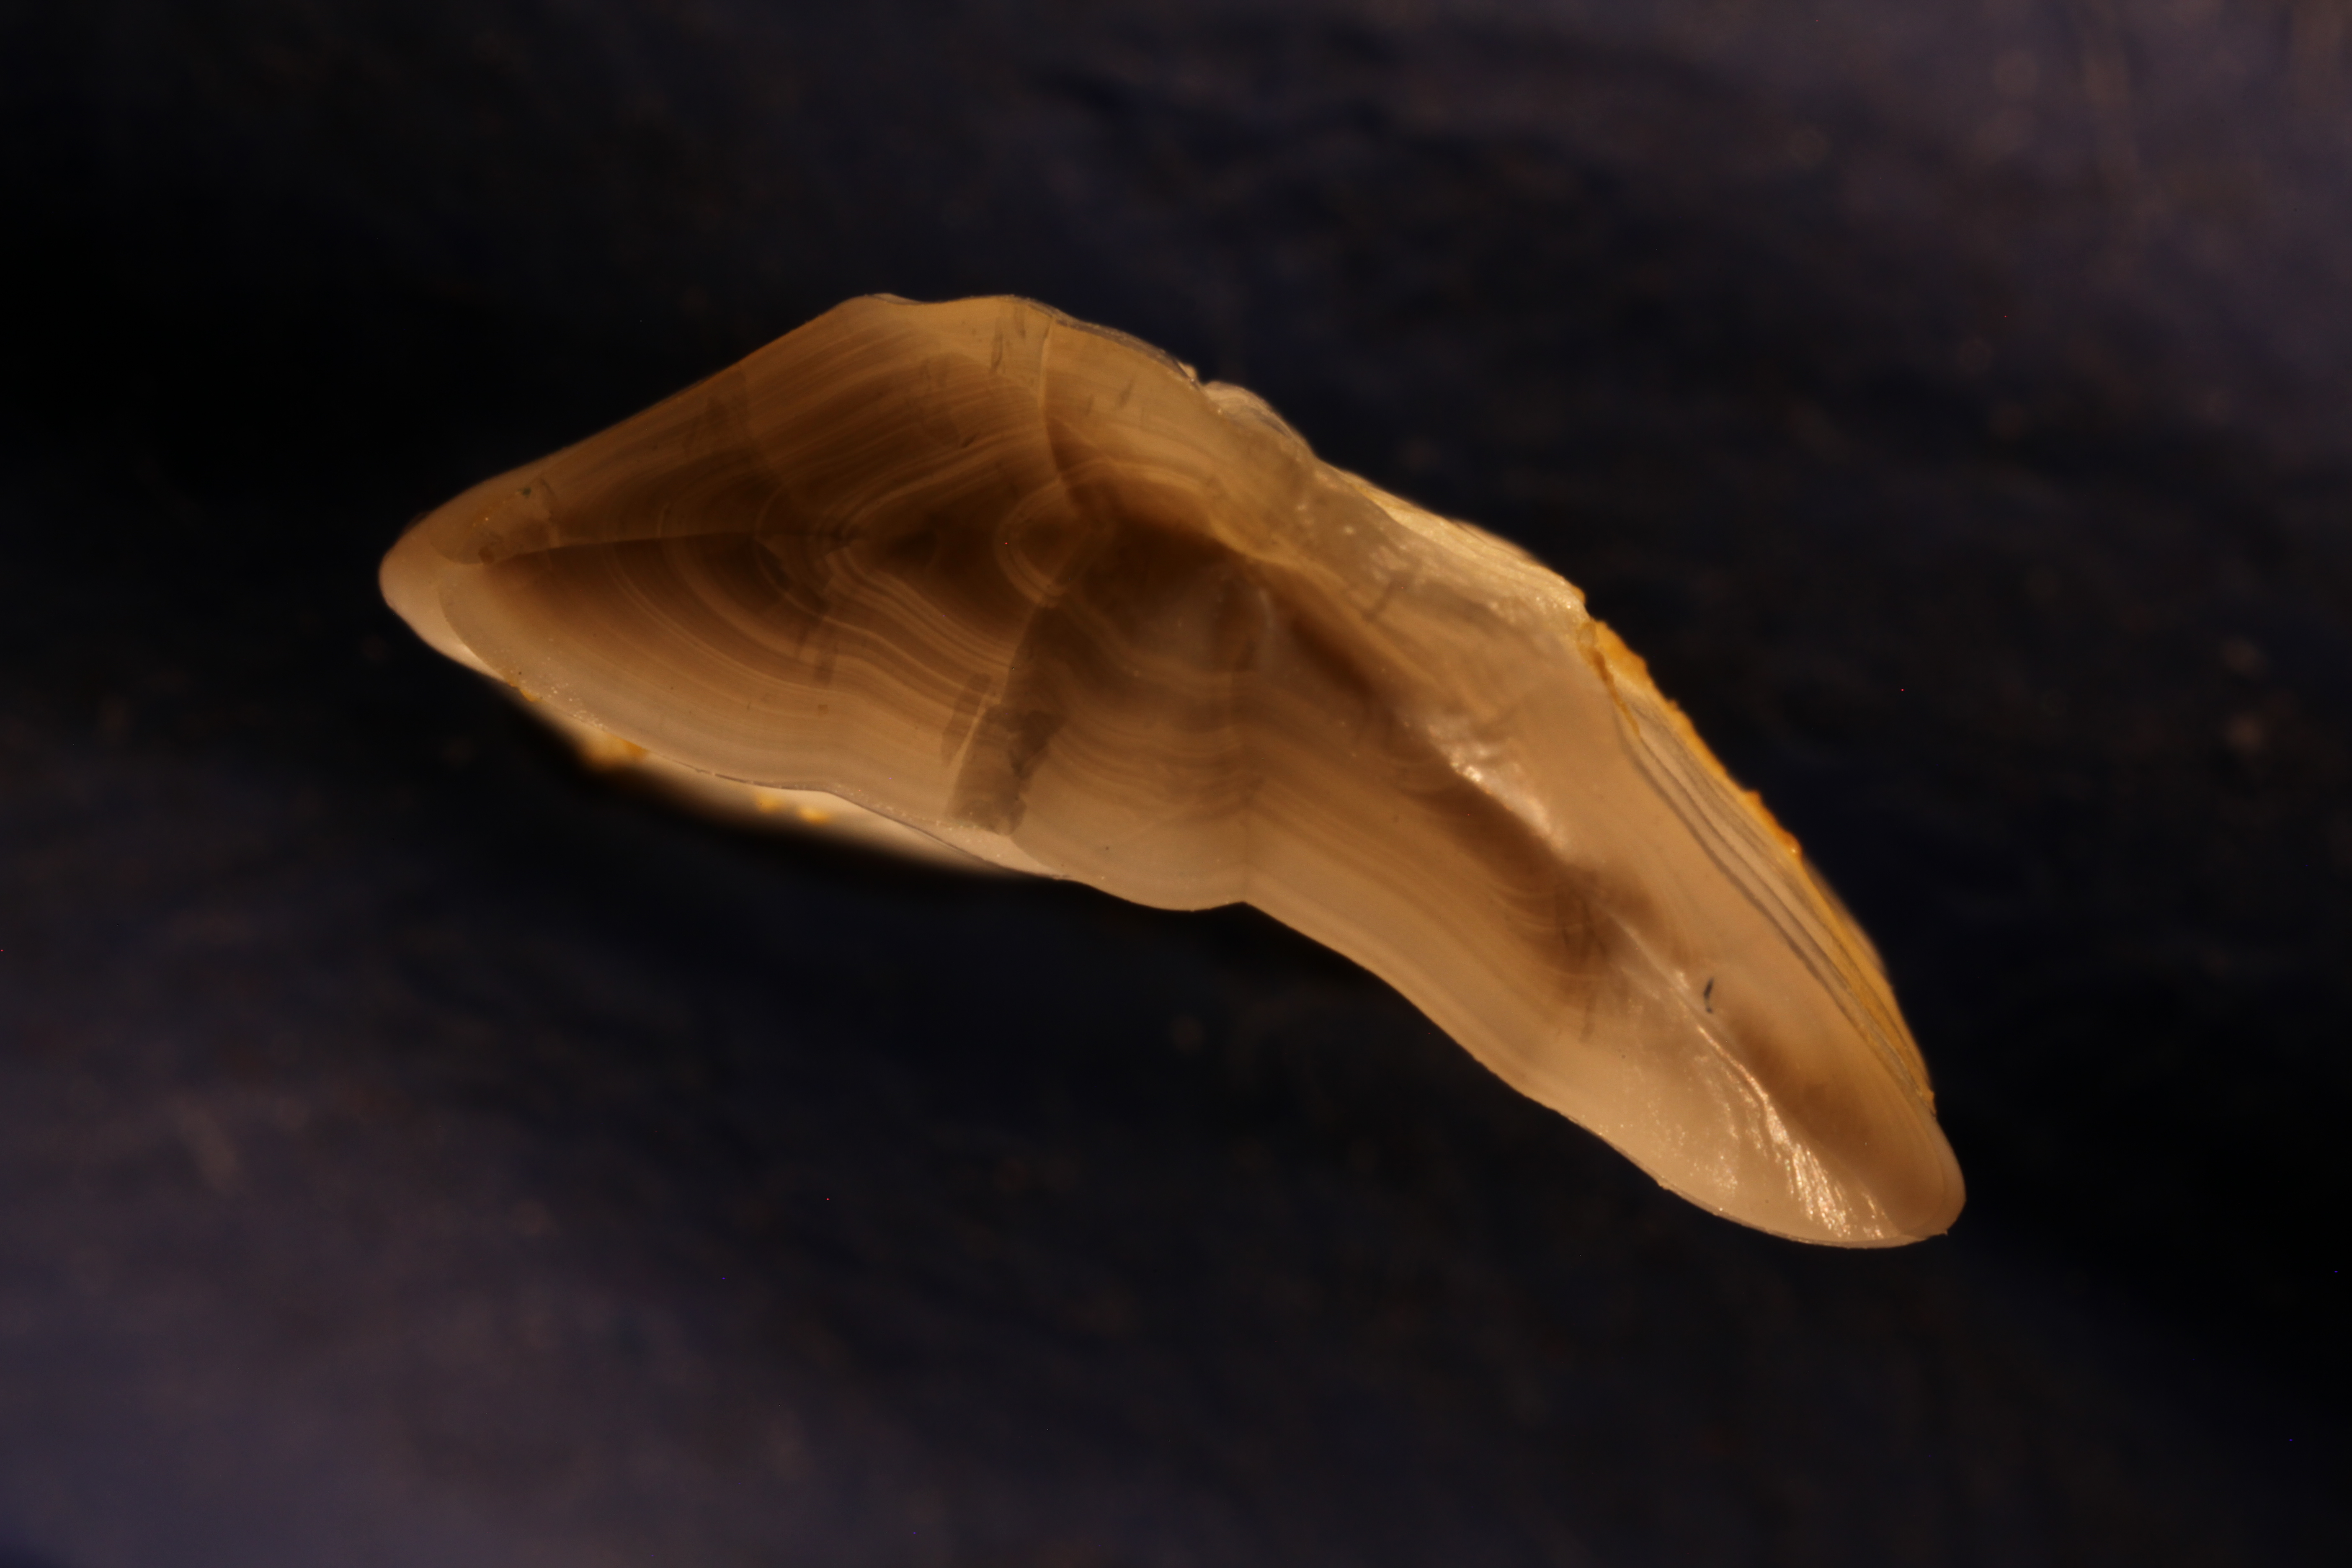
\includegraphics[scale=0.015]{otolith/IMG_0457_2016_70021.JPG}
  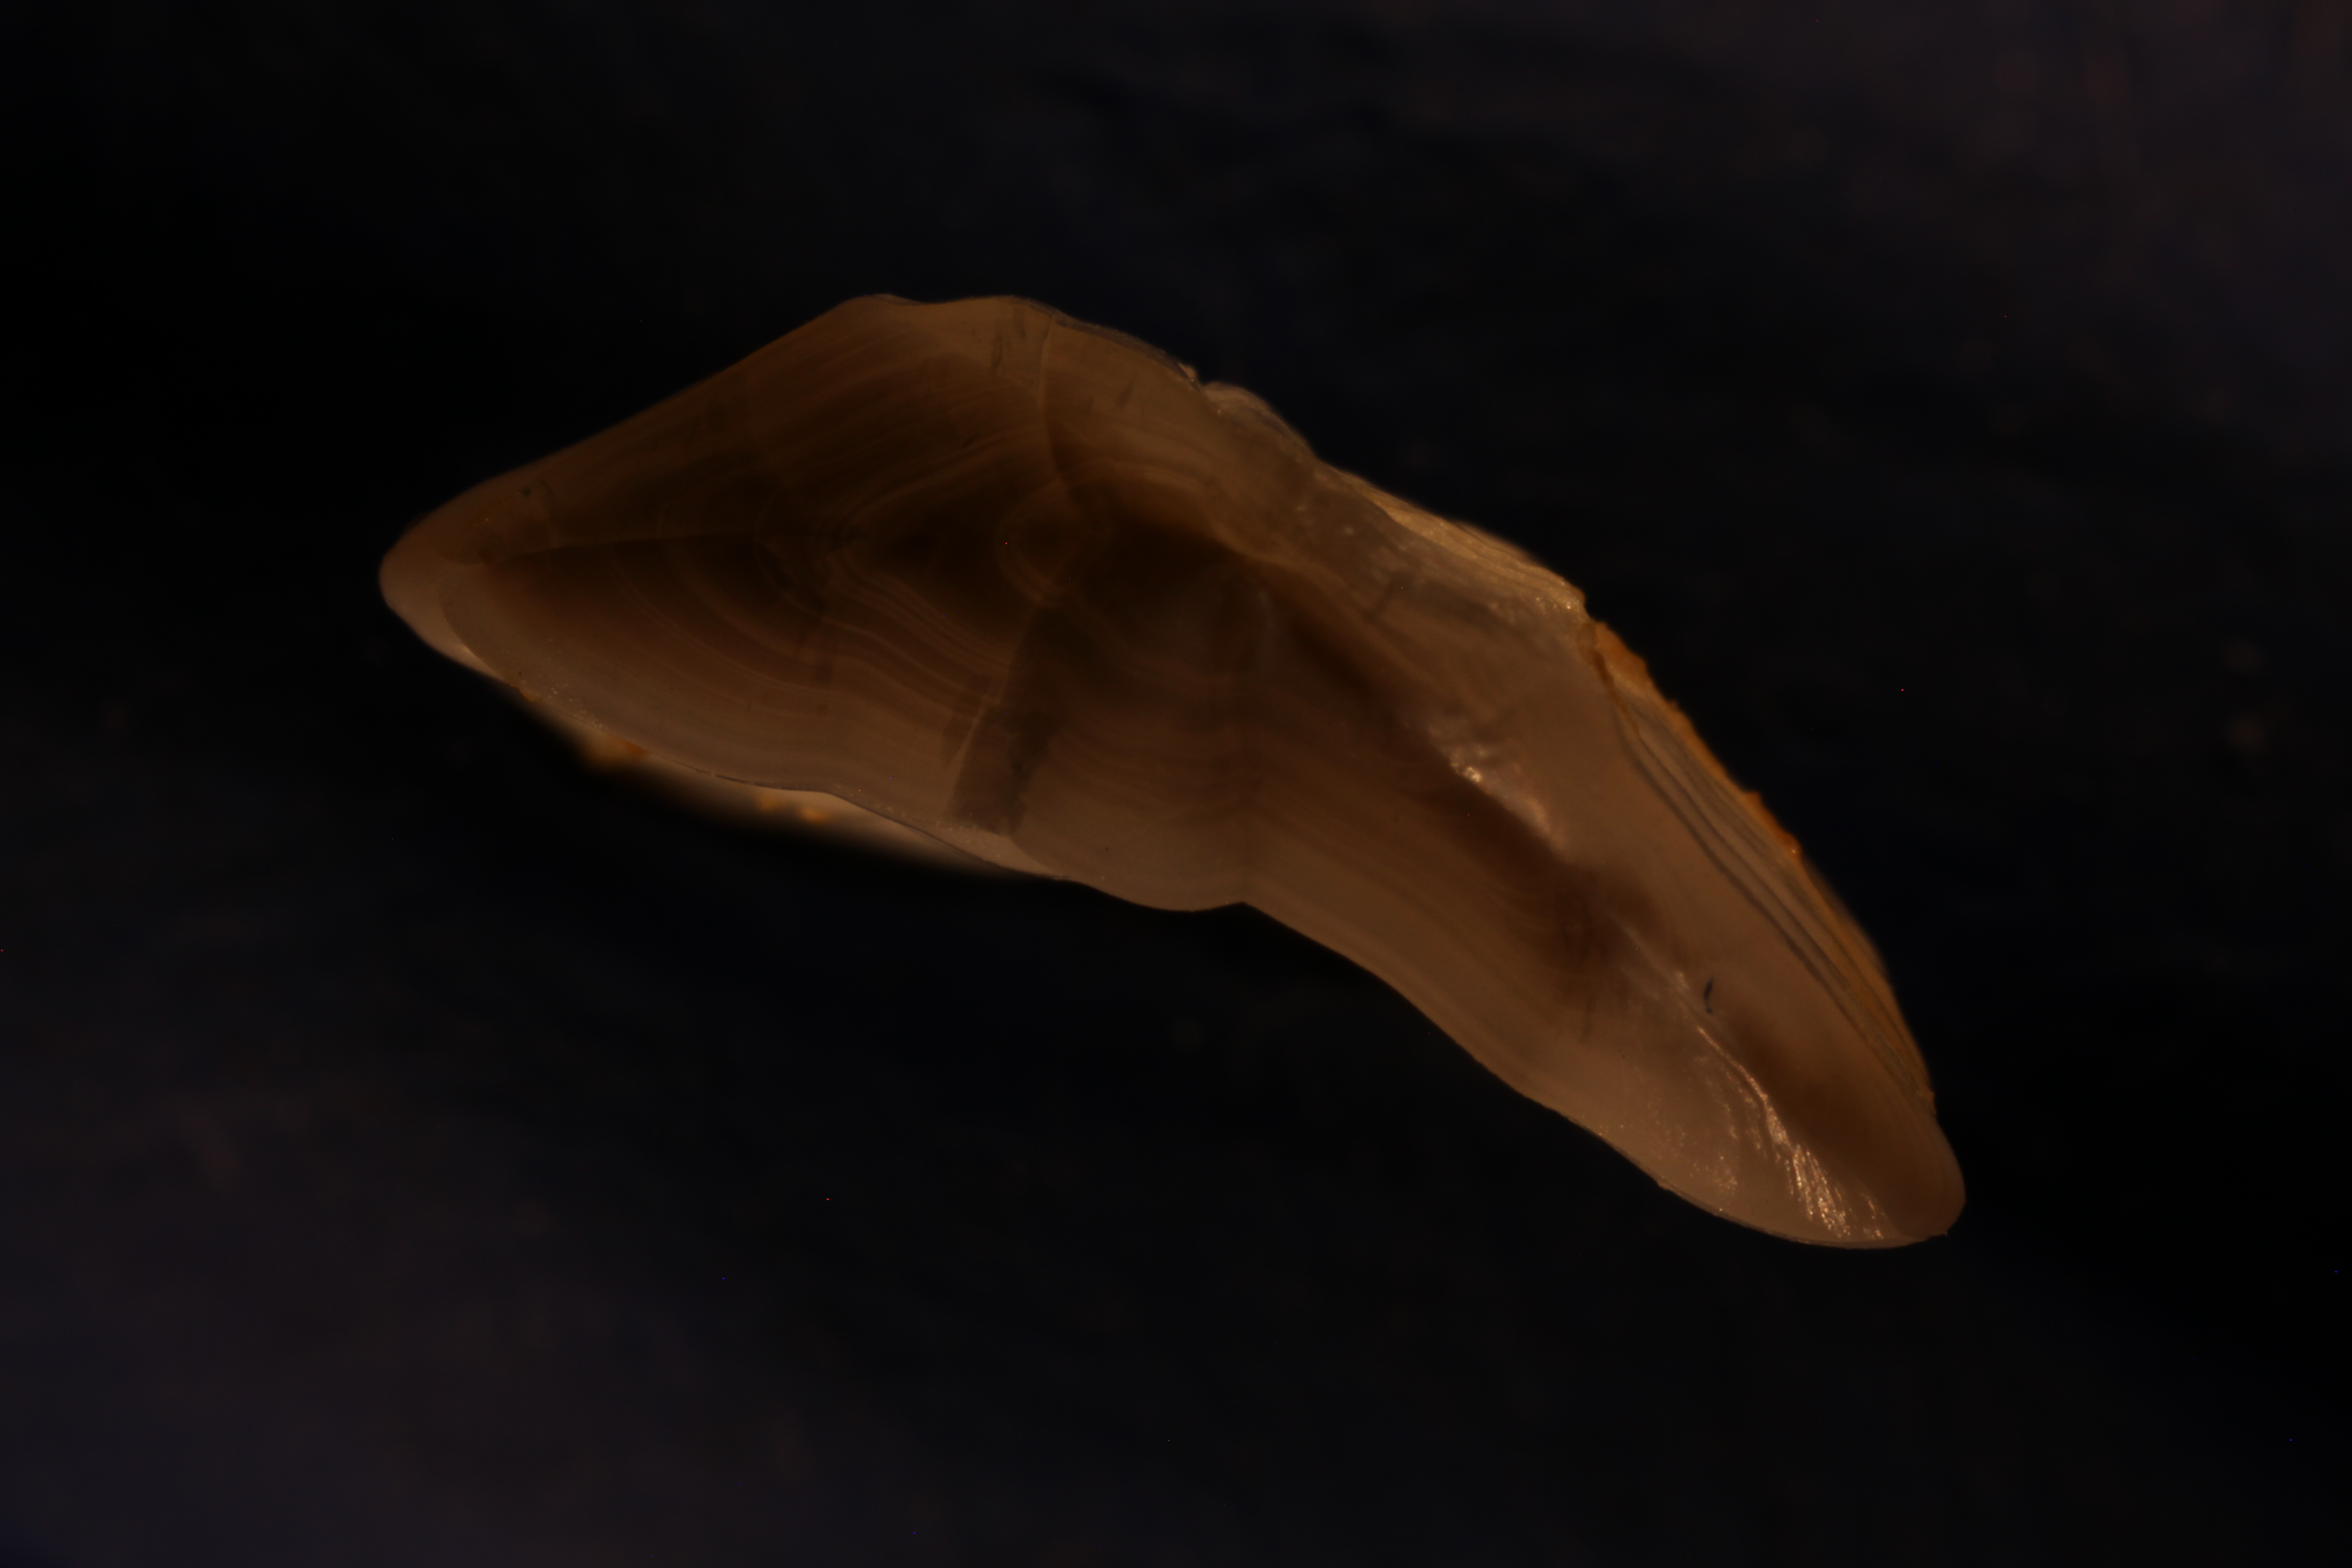
\includegraphics[scale=0.015]{otolith/IMG_0458_2016_70021.JPG}
  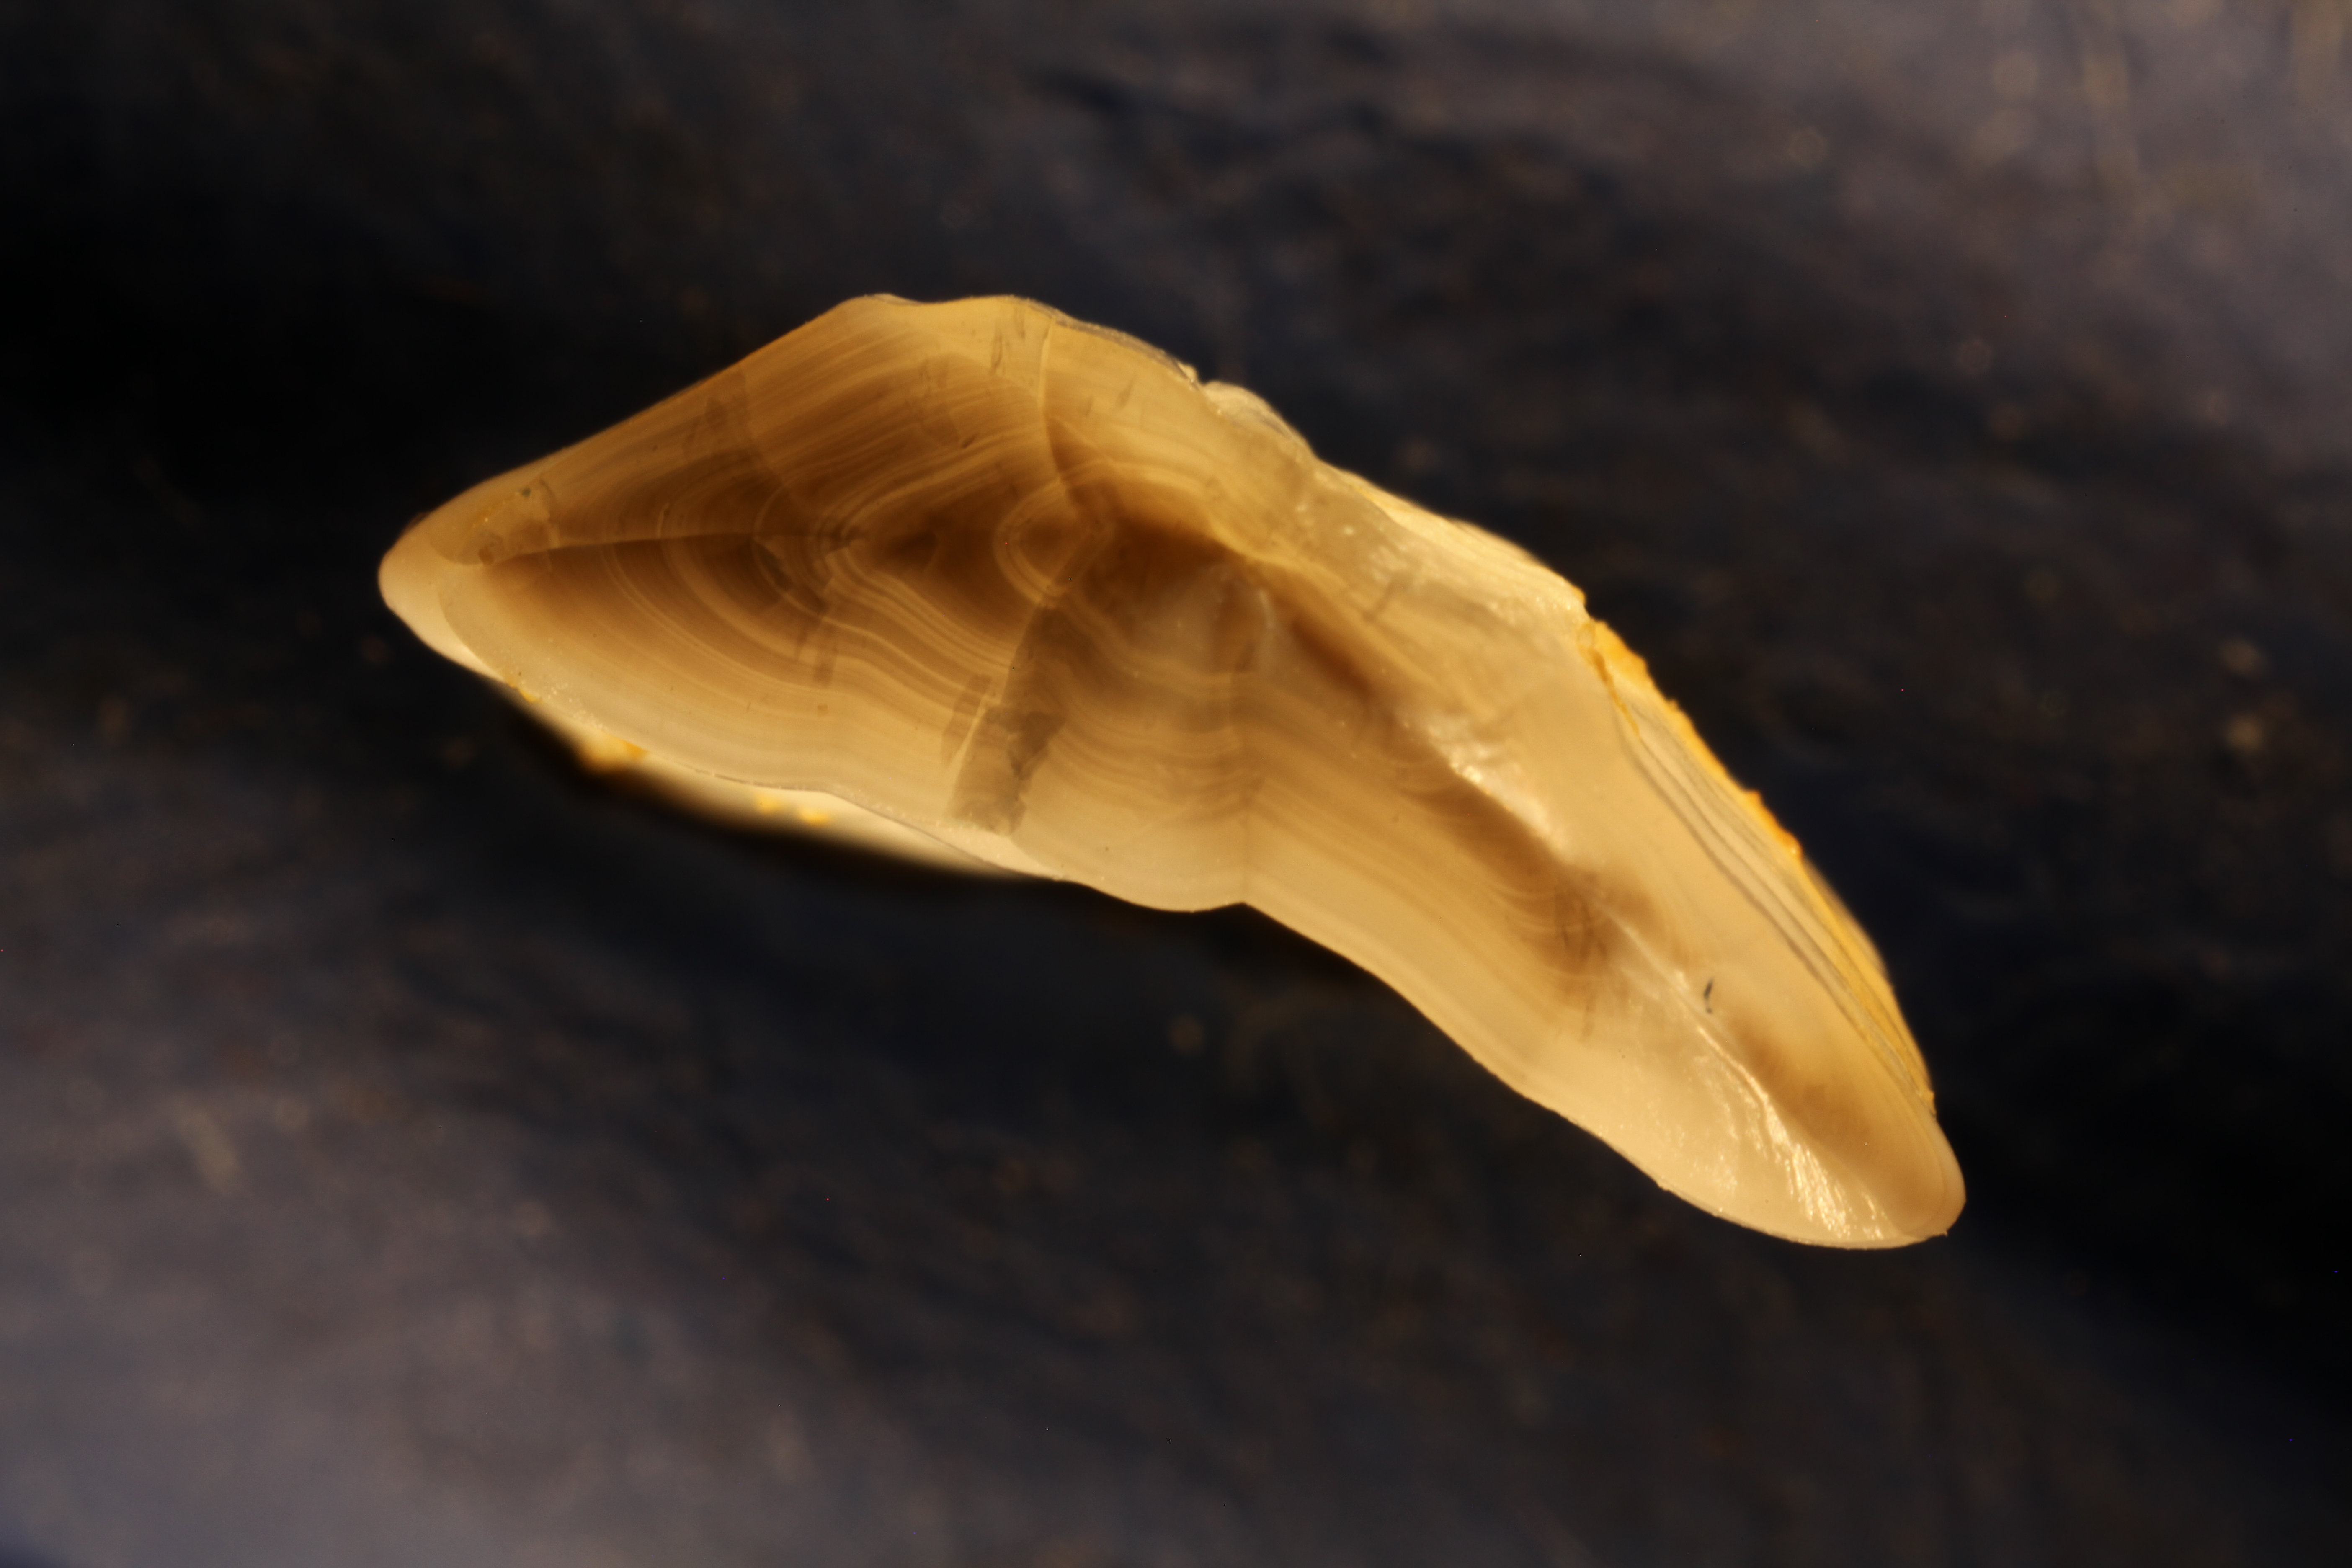
\includegraphics[scale=0.015]{otolith/IMG_0459_2016_70021.JPG} 

  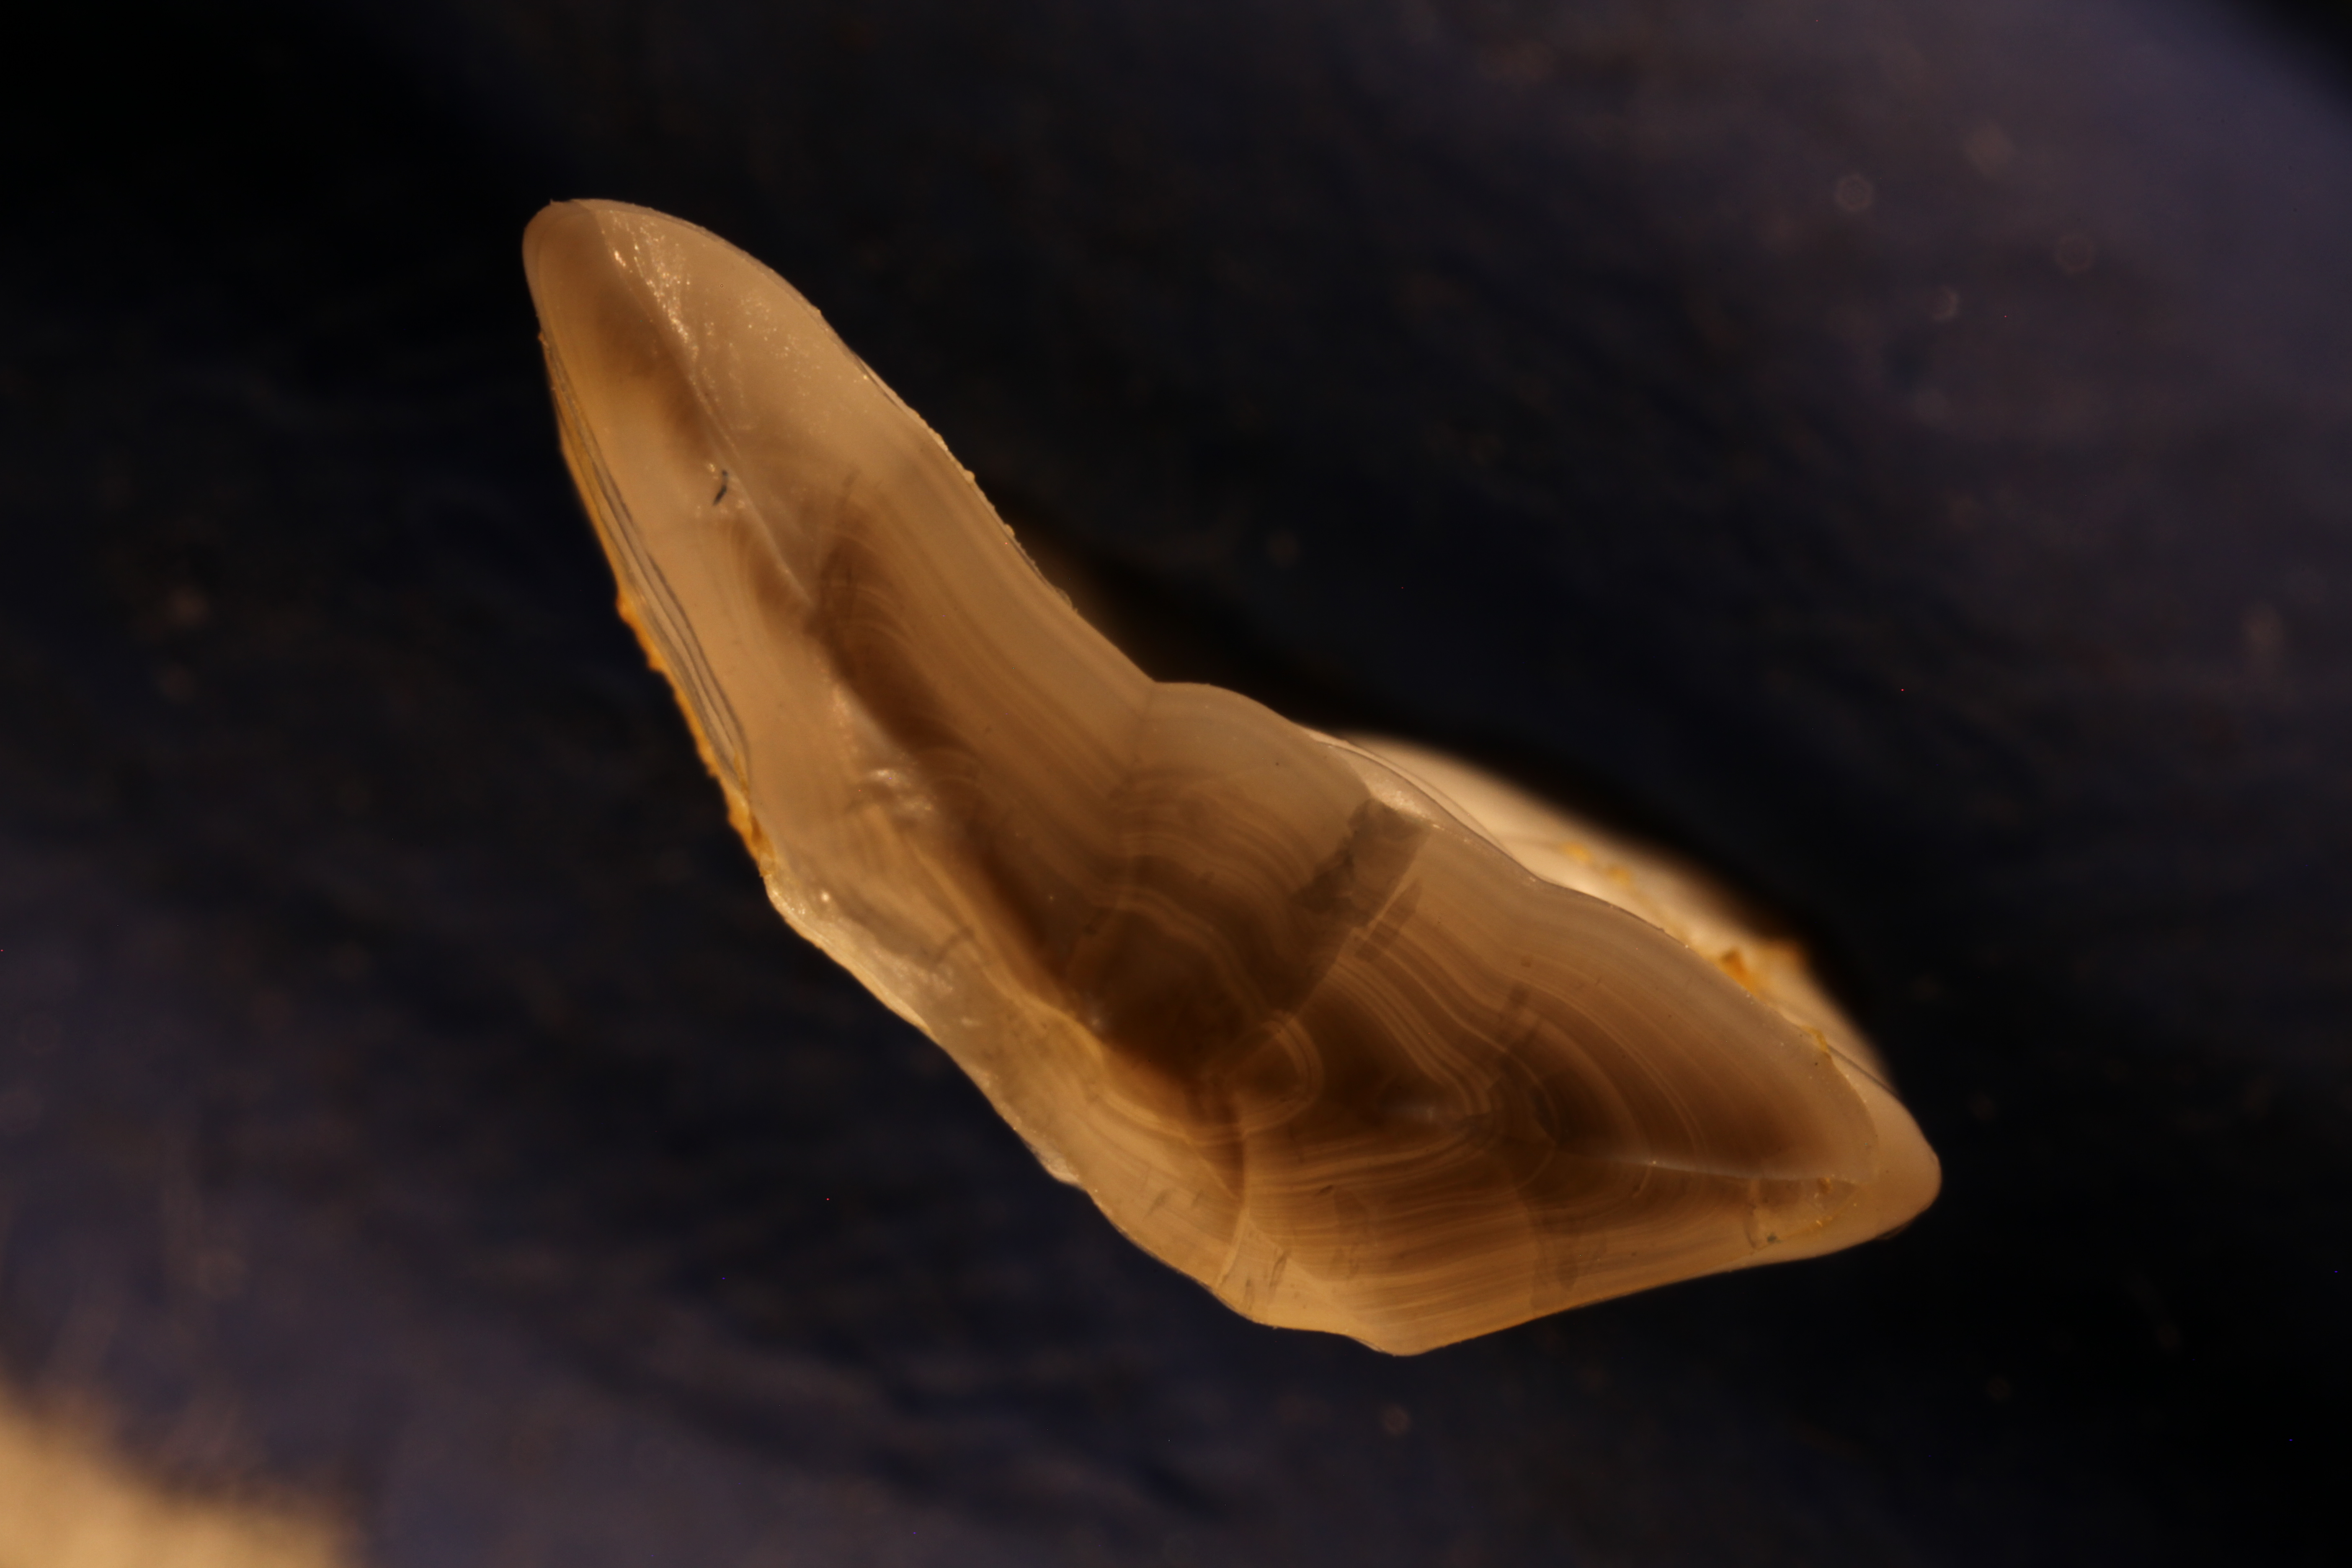
\includegraphics[scale=0.015]{otolith/IMG_0460_2016_70021.JPG}
  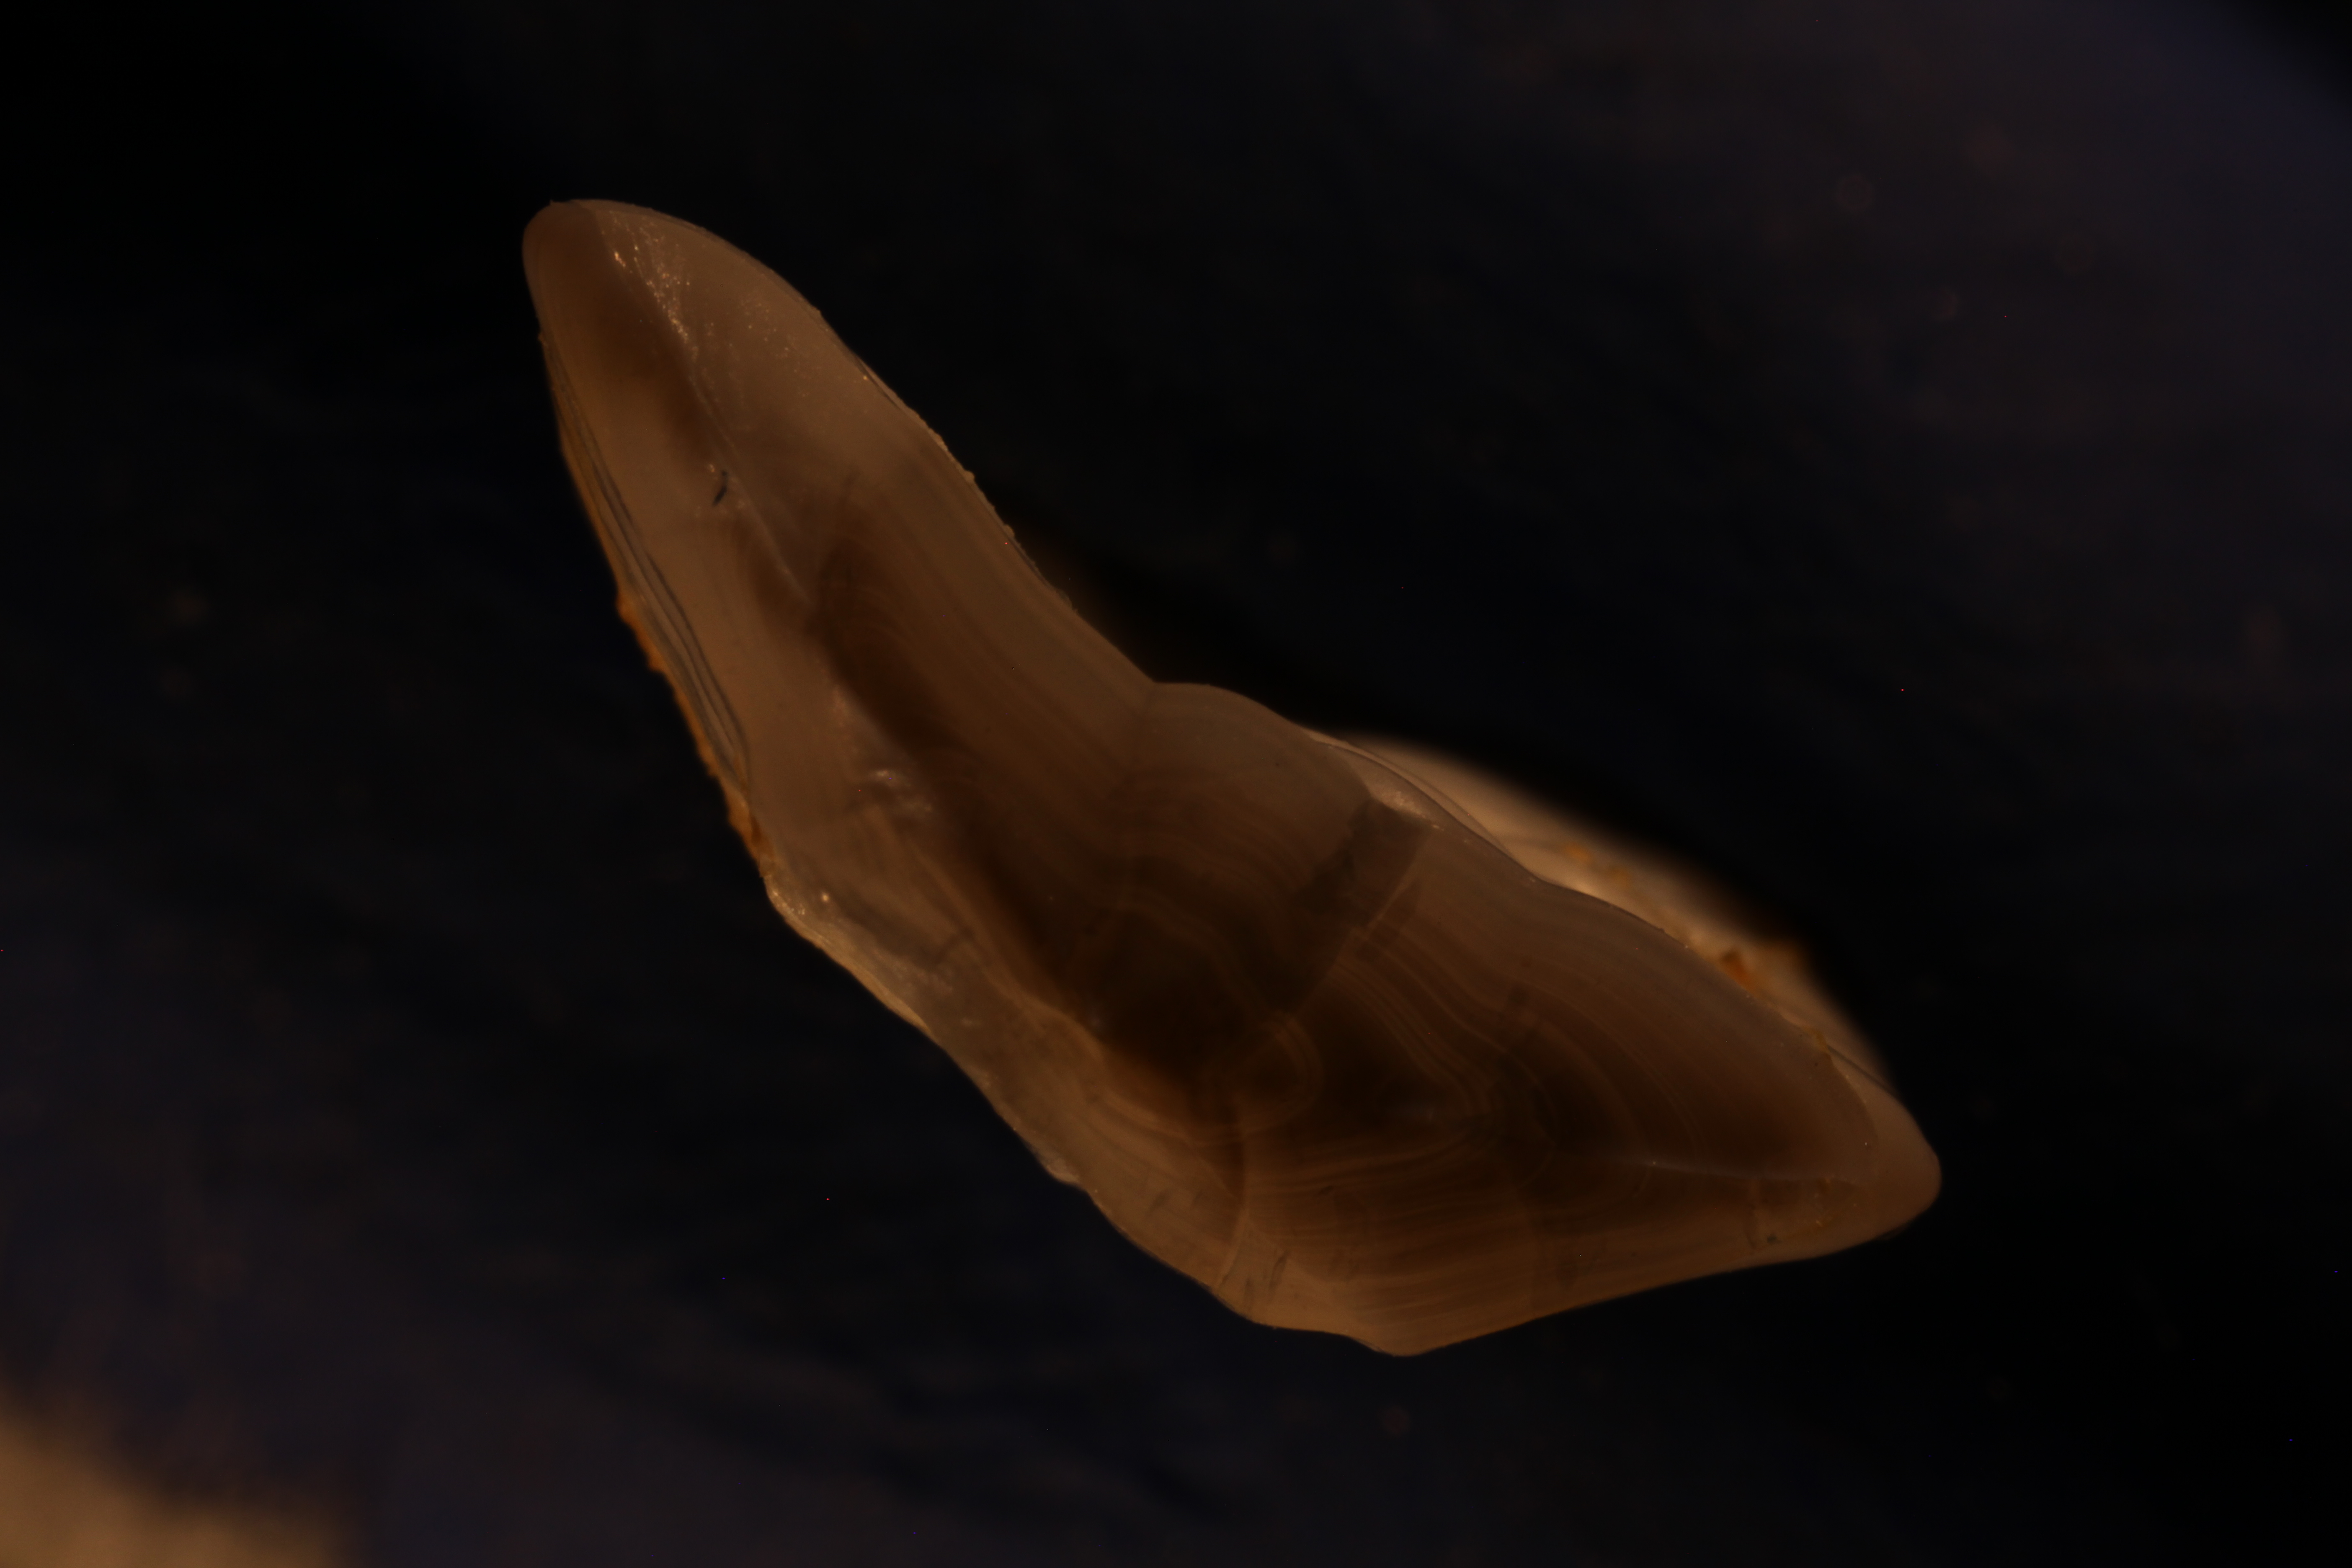
\includegraphics[scale=0.015]{otolith/IMG_0461_2016_70021.JPG}
  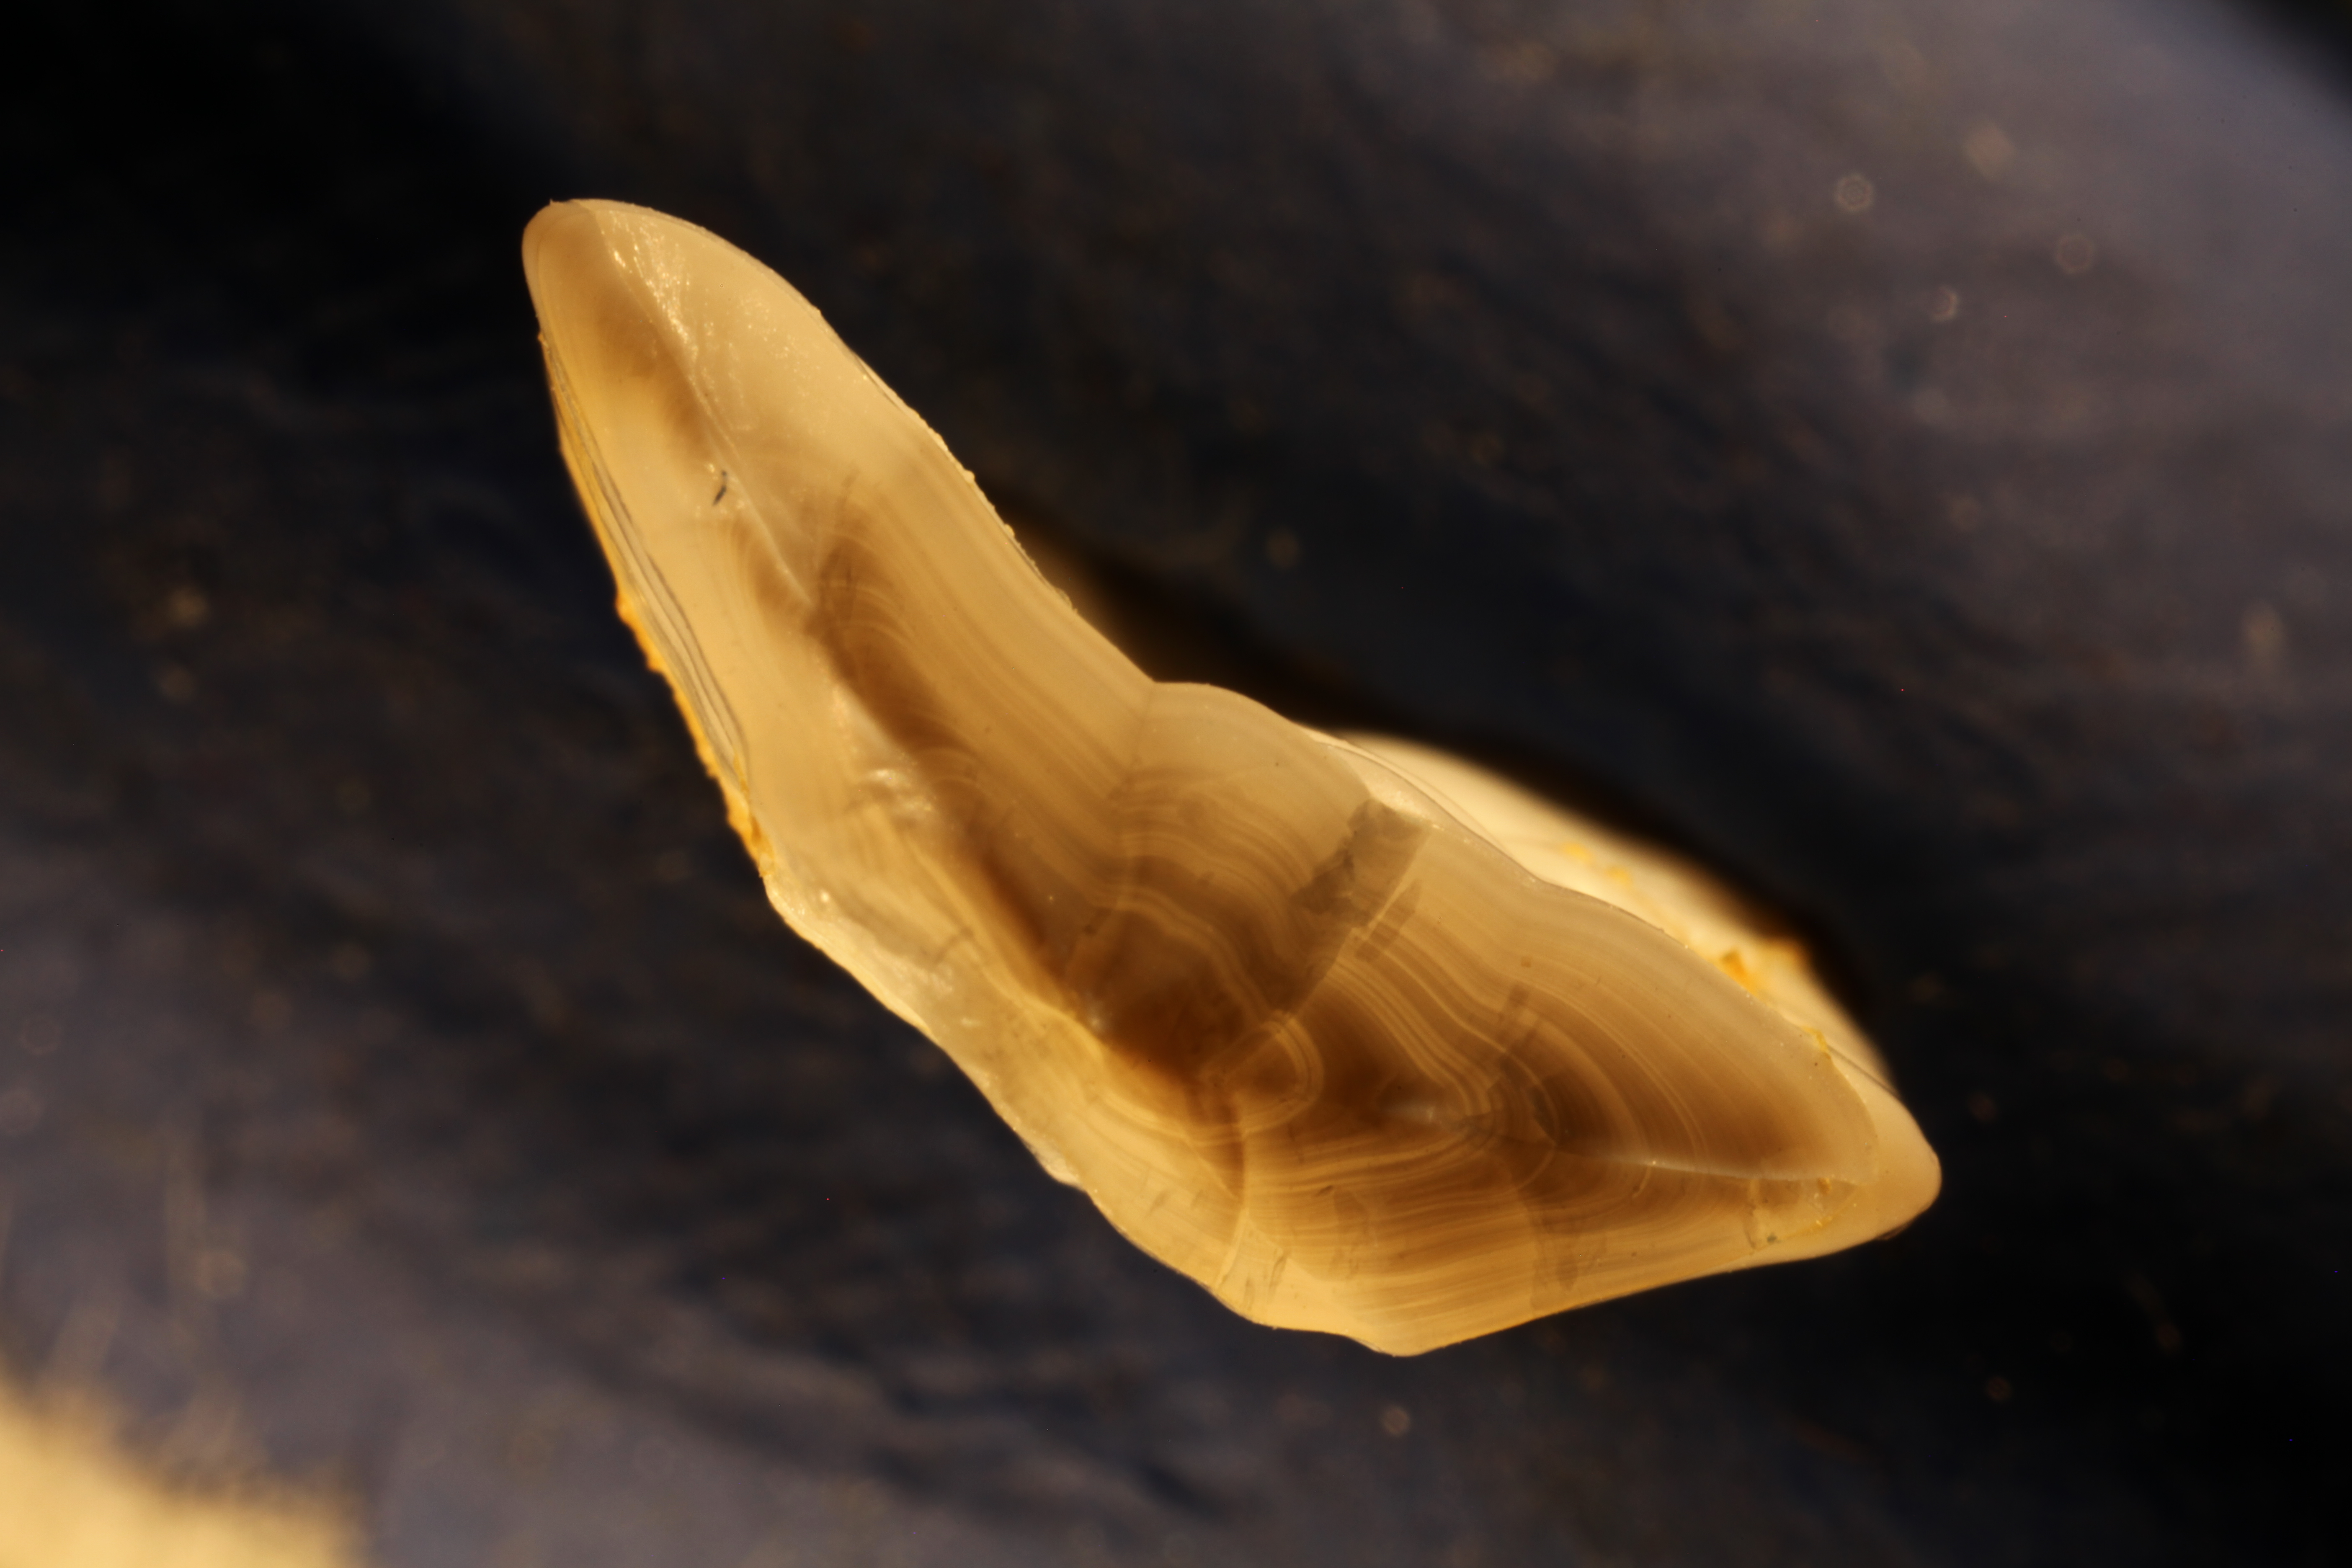
\includegraphics[scale=0.015]{otolith/IMG_0462_2016_70021.JPG}
  
  \label{marker1}
\end{figure}

"3. resulting images (size, exposures, number, method)" 

The images are 3744$\times$5616 pixels which are re-scaled for training to between 380$\times$380 to 512$\times$512. The image light exposure varies depending on light condition outside, and are stored in the metadata of the JPG file. Typically the exposure order is middle-dark-light then the rotation, and then middle-light-dark again. 
Sometimes the order is changed, so the order is recovered by reading the metadata property.

The details of how the data-set is collected and sampled from surveys, camera and mount 
setup, and how the otolith was processed before imaging, the resulting exposures, naming and
folders organization can be found in \citep{codOtolithsMyers} as well as where the data-set is available.

\begin{figure}[h!]
  \centering
  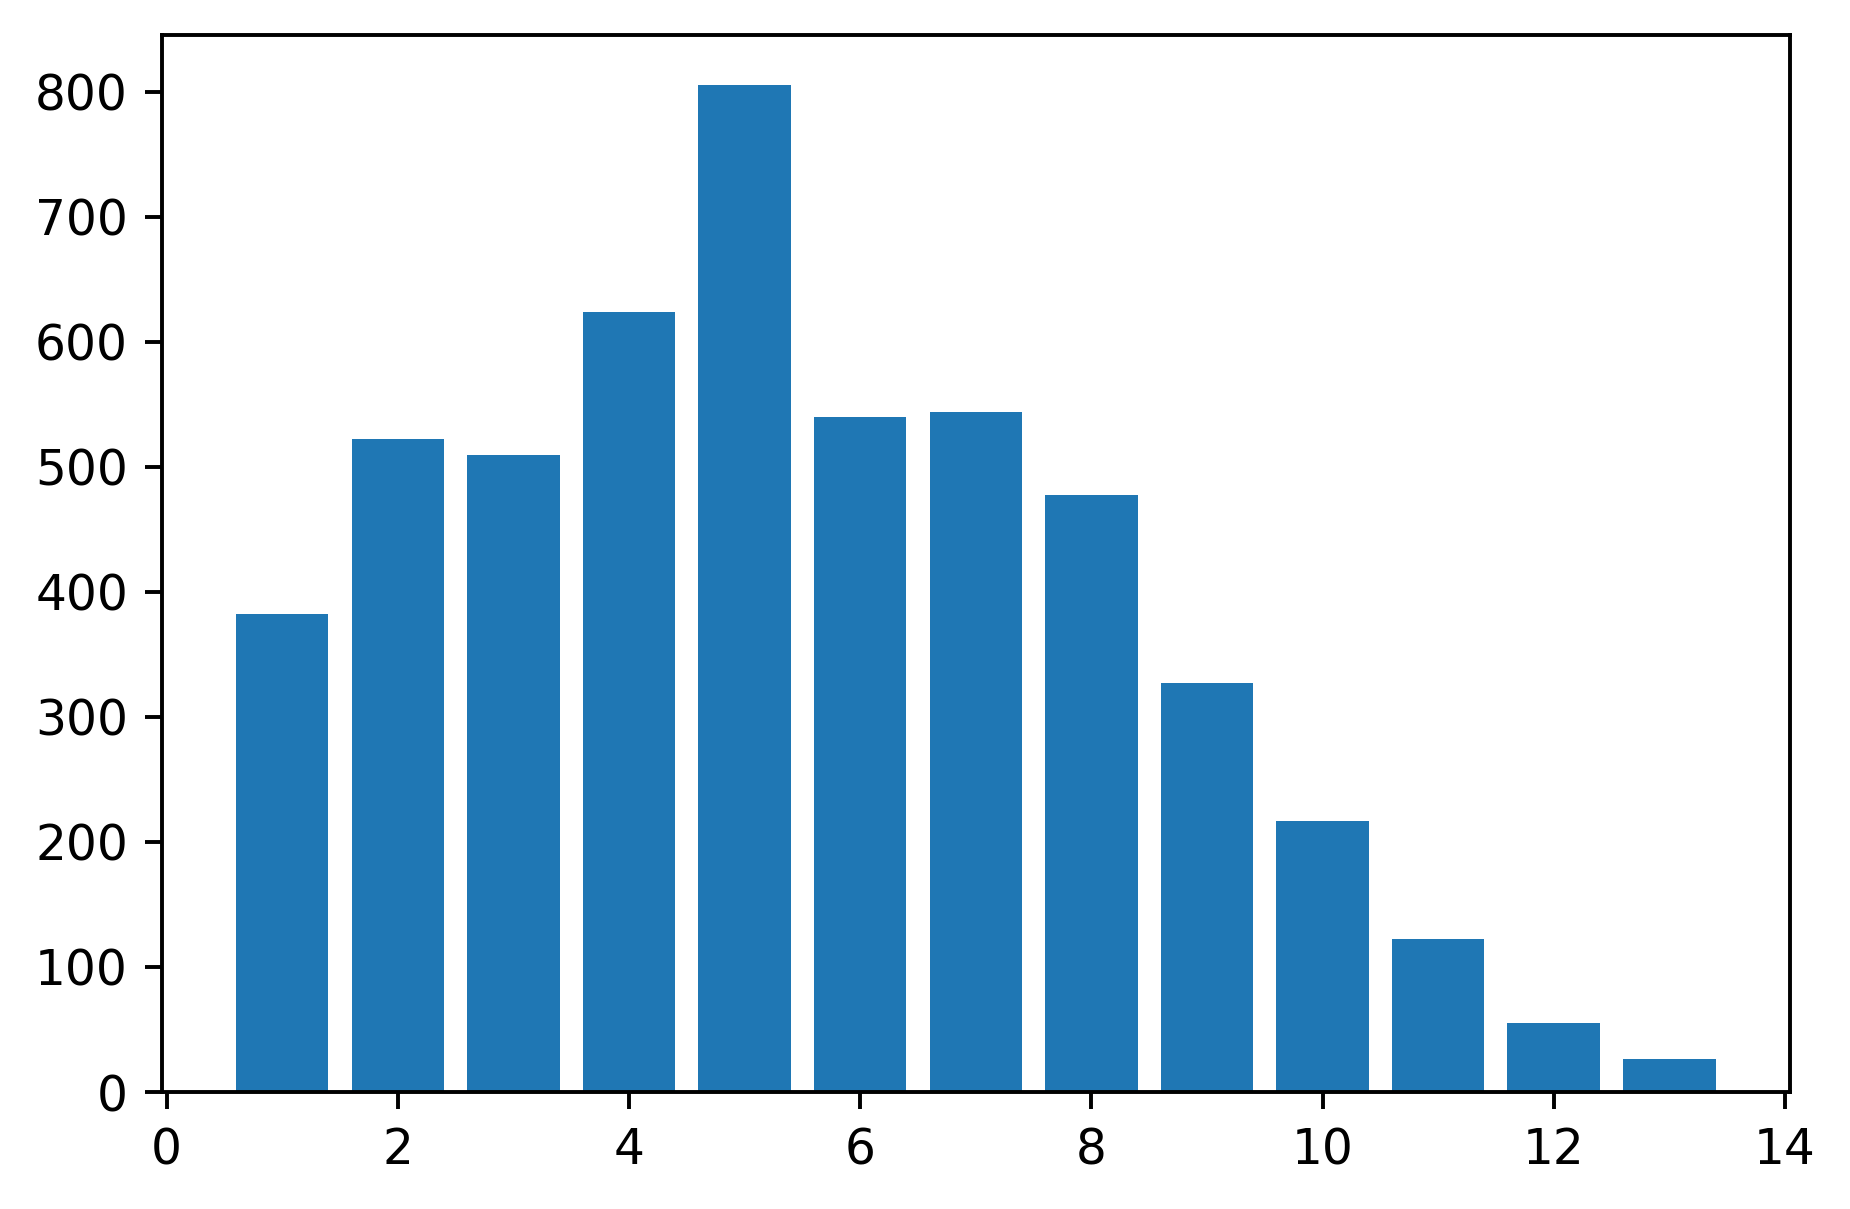
\includegraphics[scale=0.60]{distribution/age_distribution.png}
  \caption{Age distribution of all 5150 images}
\end{figure}

\begin{figure}[h!]
  \centering
  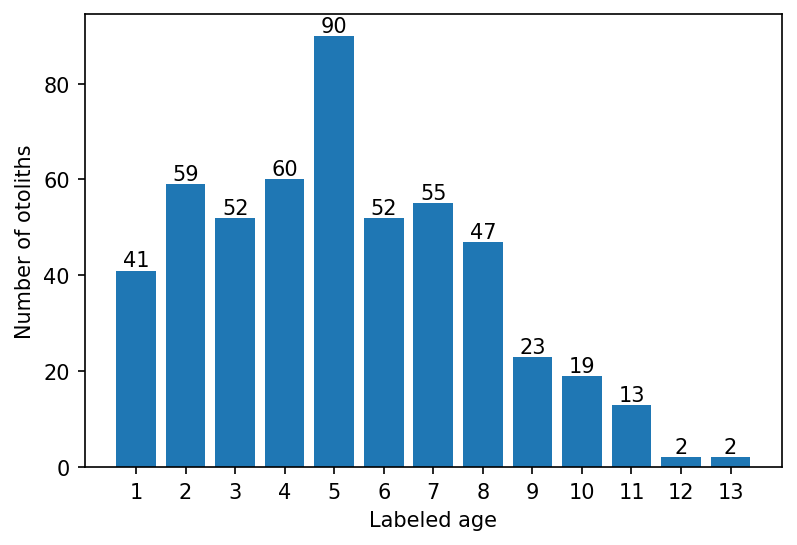
\includegraphics[scale=0.60]{distribution/age_distribution_test.png}
  \caption{Age distribution of 515 images from the test set}
\end{figure}

\subsection*{Convolutional neural network architecture}

\begin{center}
\begin{table}[hbt!]
\caption{EfficientNet and EfficientNetV2 models trained with image exposure}
\begin{tabular}{ |l|c|c|c|c|c|c| }
\hline
CNN family / & \multicolumn{3}{c|}{EfficientNet} & \multicolumn{3}{c|}{EfficientNetV2} \\
Image exposure & B4 & B5 & B6 & medium & Large  \\ 
\hline
Minimum & v & v & v & v & v  \\ 
Medium & v & v & v & v & v  \\ 
Maximum & v & v & v & v & v  \\ 
All (3 images) & x & x & x & v & v  \\ 
\hline
\end{tabular}
\label{table1}
\end{table}
\end{center}

Each CNN was trained using transfer learning by loading ImageNet  weights. The image size varies between 380$\times$380 and 528$\times$528. While test-set size prediction has been done on 380$\times$380 and 384$\times$384. To investigate the image-taking protocol described in \citep{codOtolithsMyers} we have also training on 9-channel images. Three RGB-images are stacked to produce a 9-channel image. Using Timm\citep{rw2019timm} the imageNet weights were duplicated on the input layer to accommodate 9 channels. The 3 images used are of dark, medium and light exposure of the first orientation.

CNNs was selected based on performance on the ImageNet benchmark and availability of open-source implementations with imageNet weights. The imageNet benchmark is for classification while we treat aging as a regression problem \citep{moenetal} \citep{vaboeetal}. The last layer of the CNNs has been modified to output a linear output. In the EfficientNetV2 family we have done this by applying three multi-layer perceptron layers going from 1280 output of last hidden layer to dense 256-layer, then a leakyRelu \citep{DBLP:journals/corr/XuWCL15} layer, and then dense 32-layer, then a leakyRelu layer, and finally a linear output layer. For EfficientNet we only change the last layer from softmax output to a linear output output.

To each fold we normalize the age on the training-set by removing the mean and scaling to unit variance. The normalization is then applied to validation and test-set using sklearns StandardScalar. Test-set predictions are obtained by applying the inverse transform.

\begin{figure}[h!]
  \caption{Otolith from 2013, read age: 6. With light exposure: medium, low, high, 
  and expectation per channel of the three exposures. }
  \centering
  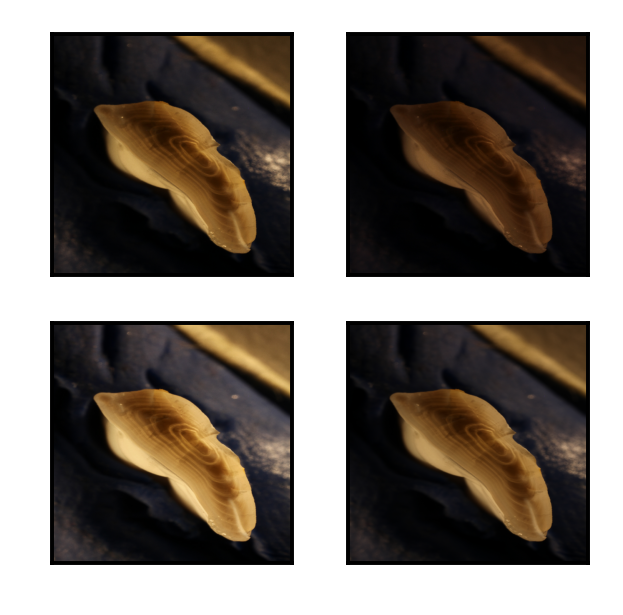
\includegraphics[scale=1.0]{otolith/2013_70174_Nr06_age09_IMG_0031_32_33.png}
  
  \label{marker2}
\end{figure}

\subsection*{Implementation and training}

EfficientNetV1 B4, B5, and B6 was implemented with  TensorFlow \citep{abadi2016tensorflow} and Keras \citep{keras} software packages in Python. Computation was done using CUDA 11.1 and CuDNN with Nvidia(Nvidia Corp., Santa Clara, California) A6000 accelerator card with 48 GB of GPU memory,
EfficientNetV2 medium, and large was implemented with the PyTorch \citep{NEURIPS2019_9015}  and timm \citep{rw2019timm} software package. Computation was done on P100 cards with 12 GB of GPU memory and RTX 3090 with 24 GB of GPU memory. Pretrained weights for EfficientNet was available from Keras, and pretrained weights for EfficeintNetV2 was available from timm.

Augmentation was applied to the training-set. The images were augmented using rotation between 0 and 360 degrees, and reflection by the vertical axis. The pixel values has a range between 0 and 255 which was normalized to between 0 and 1.

The augmented data set can produce 360$\times$2$\times$5150 = 3.708.000 possible images.
Depending on the augmentation factor and the number of images in a training cycle, the model will likely never see the same image twice.

The cost-function is mean squared error (MSE)
while the primary metric used for evaluating the models and comparing it to expert readers is accuracy. Accuracy is obtained by rounding the floating point number predictions to nearest integer and comparing the age classification against the true labels.
To reach human level accuracy a score of 85\% or higher is required \citep{ref_needed}.

To get the most out of a small data-set we applied 10-fold cross-validation on 90\% of the data-set, 4635 otoliths. Each fold of the 10 folds consists of 90\% of the cross-validation set and 81\% of the whole data-set, 4172 otoliths for training. Each fold had then 463 otoliths for validation which is 10\% of the cross-validation set, and 9\% of the whole data-set. Each model is training on the 4172 otoliths and the model with the best MSE on the 463 otoliths in the validation set is chosen. The best model on the validation set was then used to predict the age on the test-set, and the metric for accuracy and MSE was recorded. The test-set is chosen at random, while the 10-fold split is chosen using stratified-kfold split which preserves a similar distribution of the whole cross-validation set in each validation set. That means the 463 images in the validation-set will have similar age distribution to that of the 4635 images in the cross-validation set. Both the test-set and the whole data-set follows a normal distribution with largest age-class being 5-year-olds.

\subsection*{Hyper-parameters}

The CNN hyper-parameters configurations varies a little between the two families of networks, 
but are kept the same within the families. Some hyper-parameters
that has been tuned are batch size, learning rate, k-fold size, weight decay, step size, number of epochs, early stopping, and patience. Some parameters are constrained by the GPU memory, like batch-size which
is kept at 8 except for the B6 model which was run on the large A6000 GPU.

EfficientNet uses learning-rate with no scheduler while EfficientNetV2 
uses Cosine Annealing scheduler \citep{Loshchilov_et_al}. The training- and validation 
image size is as described in the papers except for large which uses smaller validation image size. The exact configuration of each network is available with each network result in the github page of the project (https://github.com/emoen/Deep-learning-for-regression-of-cod-otoliths).
\begin{center}
\begin{table}[hbt!]
\caption{Hyper-parameters on each model}
\begin{tabular}{ |l|c|c|c|c|c| } \hline
Param/CNN & B4 & B5 & B6 & Medium & Large  \\ \hline
\texttt{train\char`_batch\char`_size} & 8 & 8 & 16 & 8 & 8 \\ 
\texttt{img\char`_size} & 380 & 456 & 528 & 384 & 384 \\
\texttt{val\char`_img\char`_size} & 380 & 456 & 528 & 384 & 384 \\
\texttt{steps\char`_per\char`_epoch} & 1600 & 1600 & 1600 & 160 & (1600,160,1600,160)\\
\texttt{epochs} & 150 & 150 & (150,250x2) & 450 & (450,250,-,450) \\
\texttt{early\char`_stopping} & - & - & - & 40 & 40 \\
\texttt{early\char`_stopping\char`_patience} &  14 & 14 & (14,22,22) & - & - \\
\texttt{reduceLROnPlateau\char`_patience} & 7 & 7 & (7,11,11) & - &  - \\
\hline
\end{tabular}
\label{table2}
\end{table}
\end{center}

\begin{center}
\begin{table}[hbt!]
\caption{Hyper-parameters on all models}
\begin{tabular}{ |l|c| } \hline
\texttt{learning\char`_rate} & 1e-05 \\
\texttt{n\char`_fold} & 10 \\
\texttt{test\char`_size} & 0.1 \\
\texttt{in\char`_chans} & 3 or 9 \\
\hline
\end{tabular}
\label{table3}
\end{table}
\end{center}

\texttt{in\char`_chans} is the number of channels as input for the model. It is either 3 for an RGB image or 9 channels for 3 images.

\begin{center}
\begin{table}[hbt!]
\caption{Hyper-parameters on TensorFlow models (B4,B5, B6)}
\begin{tabular}{ |l|c| } \hline
\texttt{reduceLROnPlateau\char`_factor} & 0.2 \\
\texttt{which\char`_exposure} & min, medium, max \\
\hline
\end{tabular}
\label{table4}
\end{table}
\end{center}

\begin{center}
\begin{table}[hbt!]
\caption{Hyper-parameters on PyTorch models (medium, large)}
\begin{tabular}{ |l|c| } \hline
\texttt{scheduler} & CosineAnnealingLR \\
\texttt{T\char`_max} & 10 \\
\texttt{min\char`_lr} & 1e-06 \\
\texttt{weight\char`_decay} & 1e-06 \\
\texttt{which\char`_exposure} & min, medium, max, all \\
\hline
\end{tabular}
\label{table5}
\end{table}
\end{center}


We trained 10 models using 10-fold cross-validation which produced an ensemble prediction based on the 
test-set prediction on the test-set. Typically the ensemble prediction is better than any single fold prediction. Ensembles are better because they improve 
performance. An ensemble can make better predictions and achieve better performance than any single contributing model, just as more
experts will produce higher accuracy in predicting a single otolith.
Robustness; An ensemble reduces the spread or dispersion of the predictions and model performance.
This result can be improved further by taking ensemble predictions of ensembles.
We look at all ensembles from tuple-ensembles, consisting of 2 models, which produces an ensemble of 20 models, and triplet-ensembles consisting of 3 models, to ensemble of all models which produces an ensemble consisting of 180 models. 
s
By choosing the best model we are over fitting to the test-set, but 
selecting a subset of the best of these ensembles should produce a candidate ensemble of ensemble which will produce the best prediction on a hold-out test-set.


\section*{Results}

In table \ref{table1} and table \ref{table2} are the accuracy and MSE metrics
for ensembled predictions on the 10 fold training. It can be observed that in the EfficientNet family,
larger networks has better MSE, while accuracy is not as correlated.
A similar pattern can be observed for the efficientNetV2 networks.
However it seems like efficientNet is better than efficientNetV2 in both metrics unlike
the results observed on the ImageNet benchmark.

\begin{center}
\begin{table}[hbt!]
\caption{Accuracy by light exposure and CNN architectures}
\begin{tabular}{ |l|c|c|c|c|c|c| }
\hline
MSE:light/CNN & B4 & B5 & B6 & Medium & Large \\ \hline
min        & 72.8* & 74.4 & 73.4 & 74.0 & -  \\ 
medium     & 71.5 & - & 74.4 & 72.4 & 71.8*  \\ 
max        & 70.9 & - & 71.5 & 71.1 & -  \\ 
9 channels & x & x & x & 74.0 & 71.7  \\ 
\hline
\end{tabular}
\label{table6}
\end{table}
\end{center}

\begin{center}
\begin{table}[hbt!]
\caption{MSE by light exposure and CNN architectures}
\begin{tabular}{ |l|c|c|c|c|c|c| }

\hline
ACC:light/CNN & B4 & B5 & B6 & Medium & Large  \\ \hline
min        & .277 & .277 & .272 & .273 & -  \\ 
medium     & .285 & - & .262 & .292 & .280  \\ 
max        & .291 & - & .305 & .290 & -  \\ 
9 channels & x & x & x & .273 & .281  \\ 
\hline
\end{tabular}
\label{table7}
\end{table}
\end{center}


\begin{figure}[h!]
  \centering
  \begin{minipage}[b]{1.0\textwidth}
  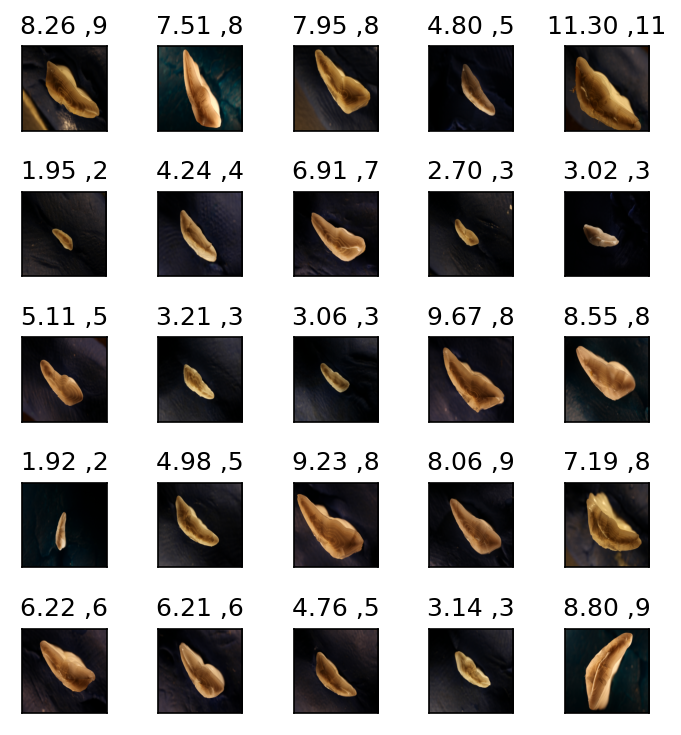
\includegraphics[scale=0.75]{results/fold_prediction_V2_m.png}
    \caption{Sample of 25 predictions on a model of training on EfficientNetV2 size medium with minimum light exposure, left number is prediction,
    and right number is age read}
   \label{marker3}
  \end{minipage}
  \hfill
\end{figure}

We compare the 10-fold prediction accuracy, and MSE of all the models in a box plot in
figure \ref{marker4}, and \ref{marker5}. The red line 
is the ensemble accuracy or MSE. The orange line is the mean accuracy or MSE. 
The ensemble metric is either better than or in the upper quantile for all the folds.

\begin{figure}[h!]
  \centering
  \begin{minipage}[b]{1.0\textwidth}
  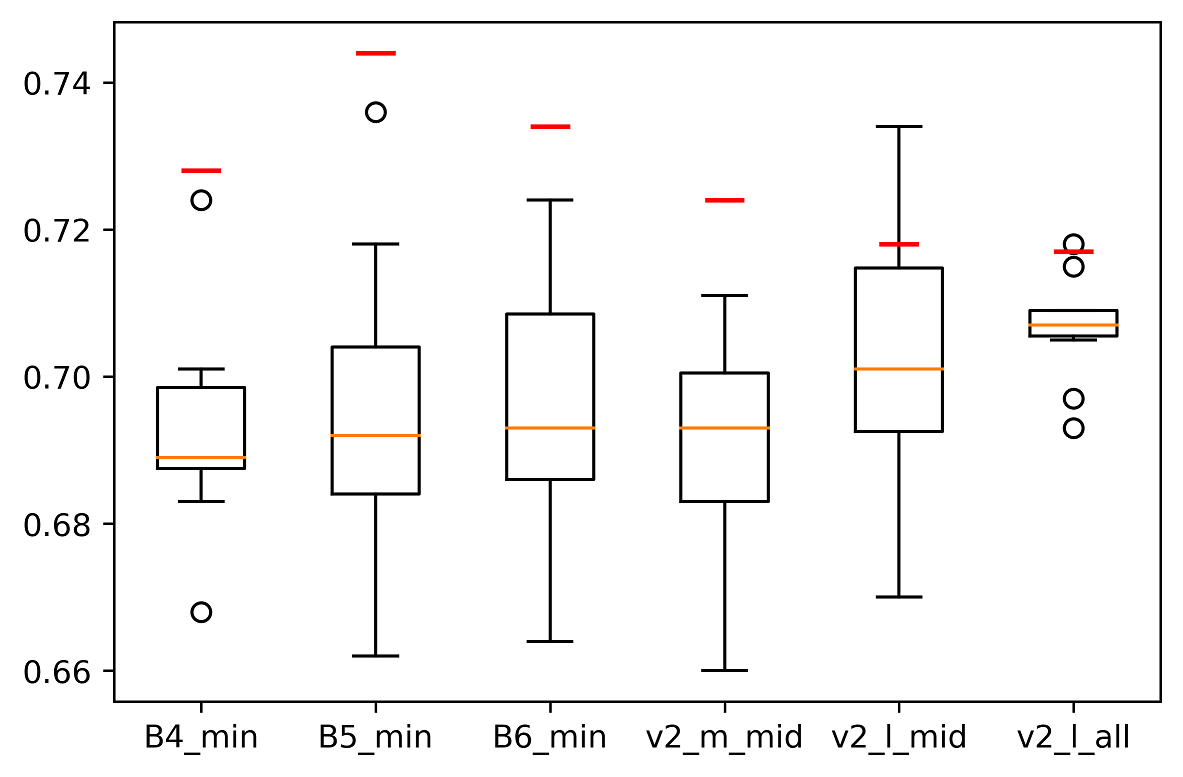
\includegraphics[scale=0.2]{results/box_plot_models_acc.png}
    \caption{Accuracy score of all the 17 models and the red line is ensemble prediction accuracy}
   \label{marker4}
  \end{minipage}
  \hfill
\end{figure}

\begin{figure}[h!]
  \centering
  \begin{minipage}[b]{0.49\textwidth}
  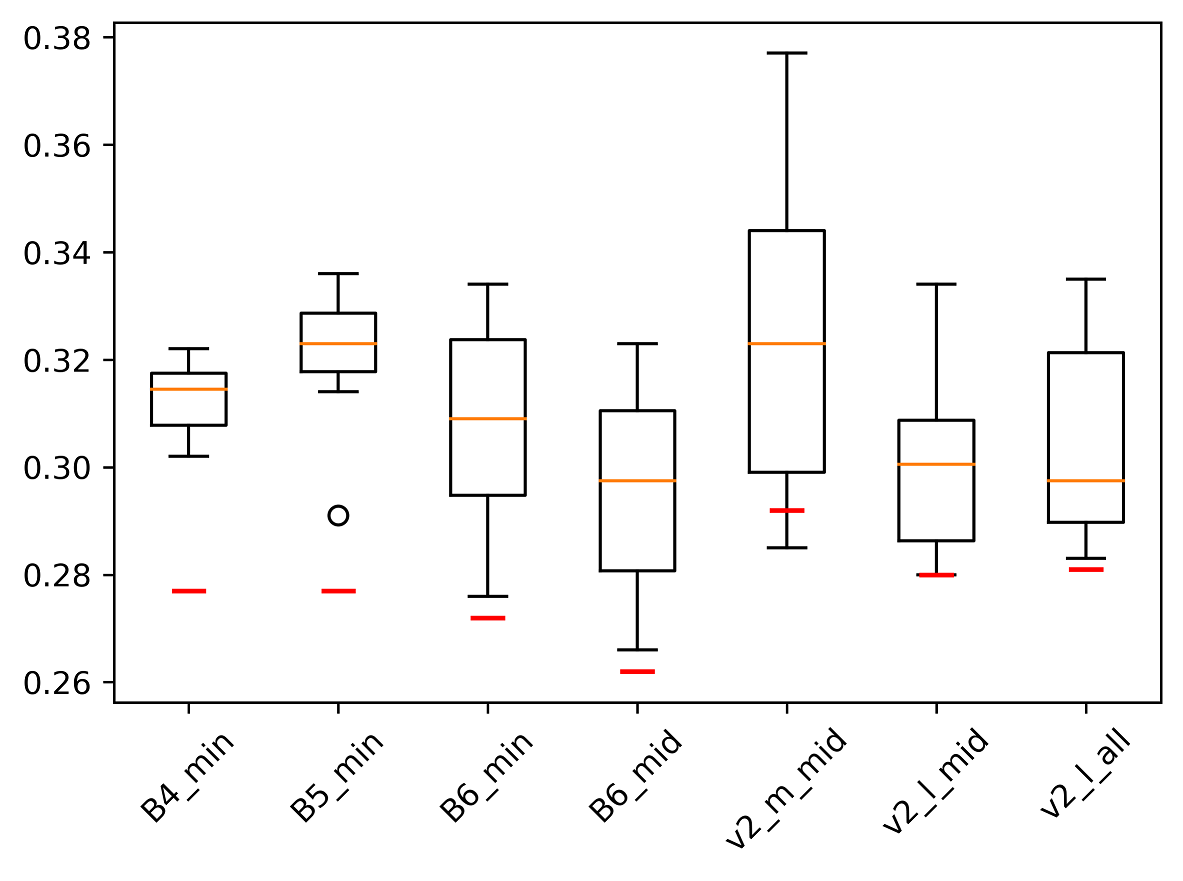
\includegraphics[scale=0.2]{results/box_plot_models_mse.png}
    \caption{MSE score of all the 17 models and the red line is ensemble prediction MSE}
   \label{marker5}
  \end{minipage}
  \hfill
\end{figure}

By comparing the models on MSE we can see that larger models are better, e.g B6 has 
higher mean than B5 and B4, and large is better than medium. 
We also see that the EfficientNetV2 networks has higher  mean than the
first generation EfficientNet. However, this is not true for the ensemble
predictions (red line) nor for the fold-mean or ensemble of the accuracy.
We can also see that the effect of adding 3 images, creating 9 channels, on the
model is that the variance is reduced, the fold mean metric increases,
but the ensemble metric is reduced.

The box plots are produced from the folds given in table \ref{table8} and \ref{table9} in appendix C

\subsection*{Prediction by age class and residuals}

Figure \ref{age_acc} shows the recidual error as the
average across all models. It looks like a normal distribution.
Assuming all age groups for all models are normal distributed,
a table with mean and standard deviation can be found in Appendix B for
each model and age-group

\begin{figure}[h!]
  \caption{Residuals per age class over all models. Red; correctly classified}
  \centering
  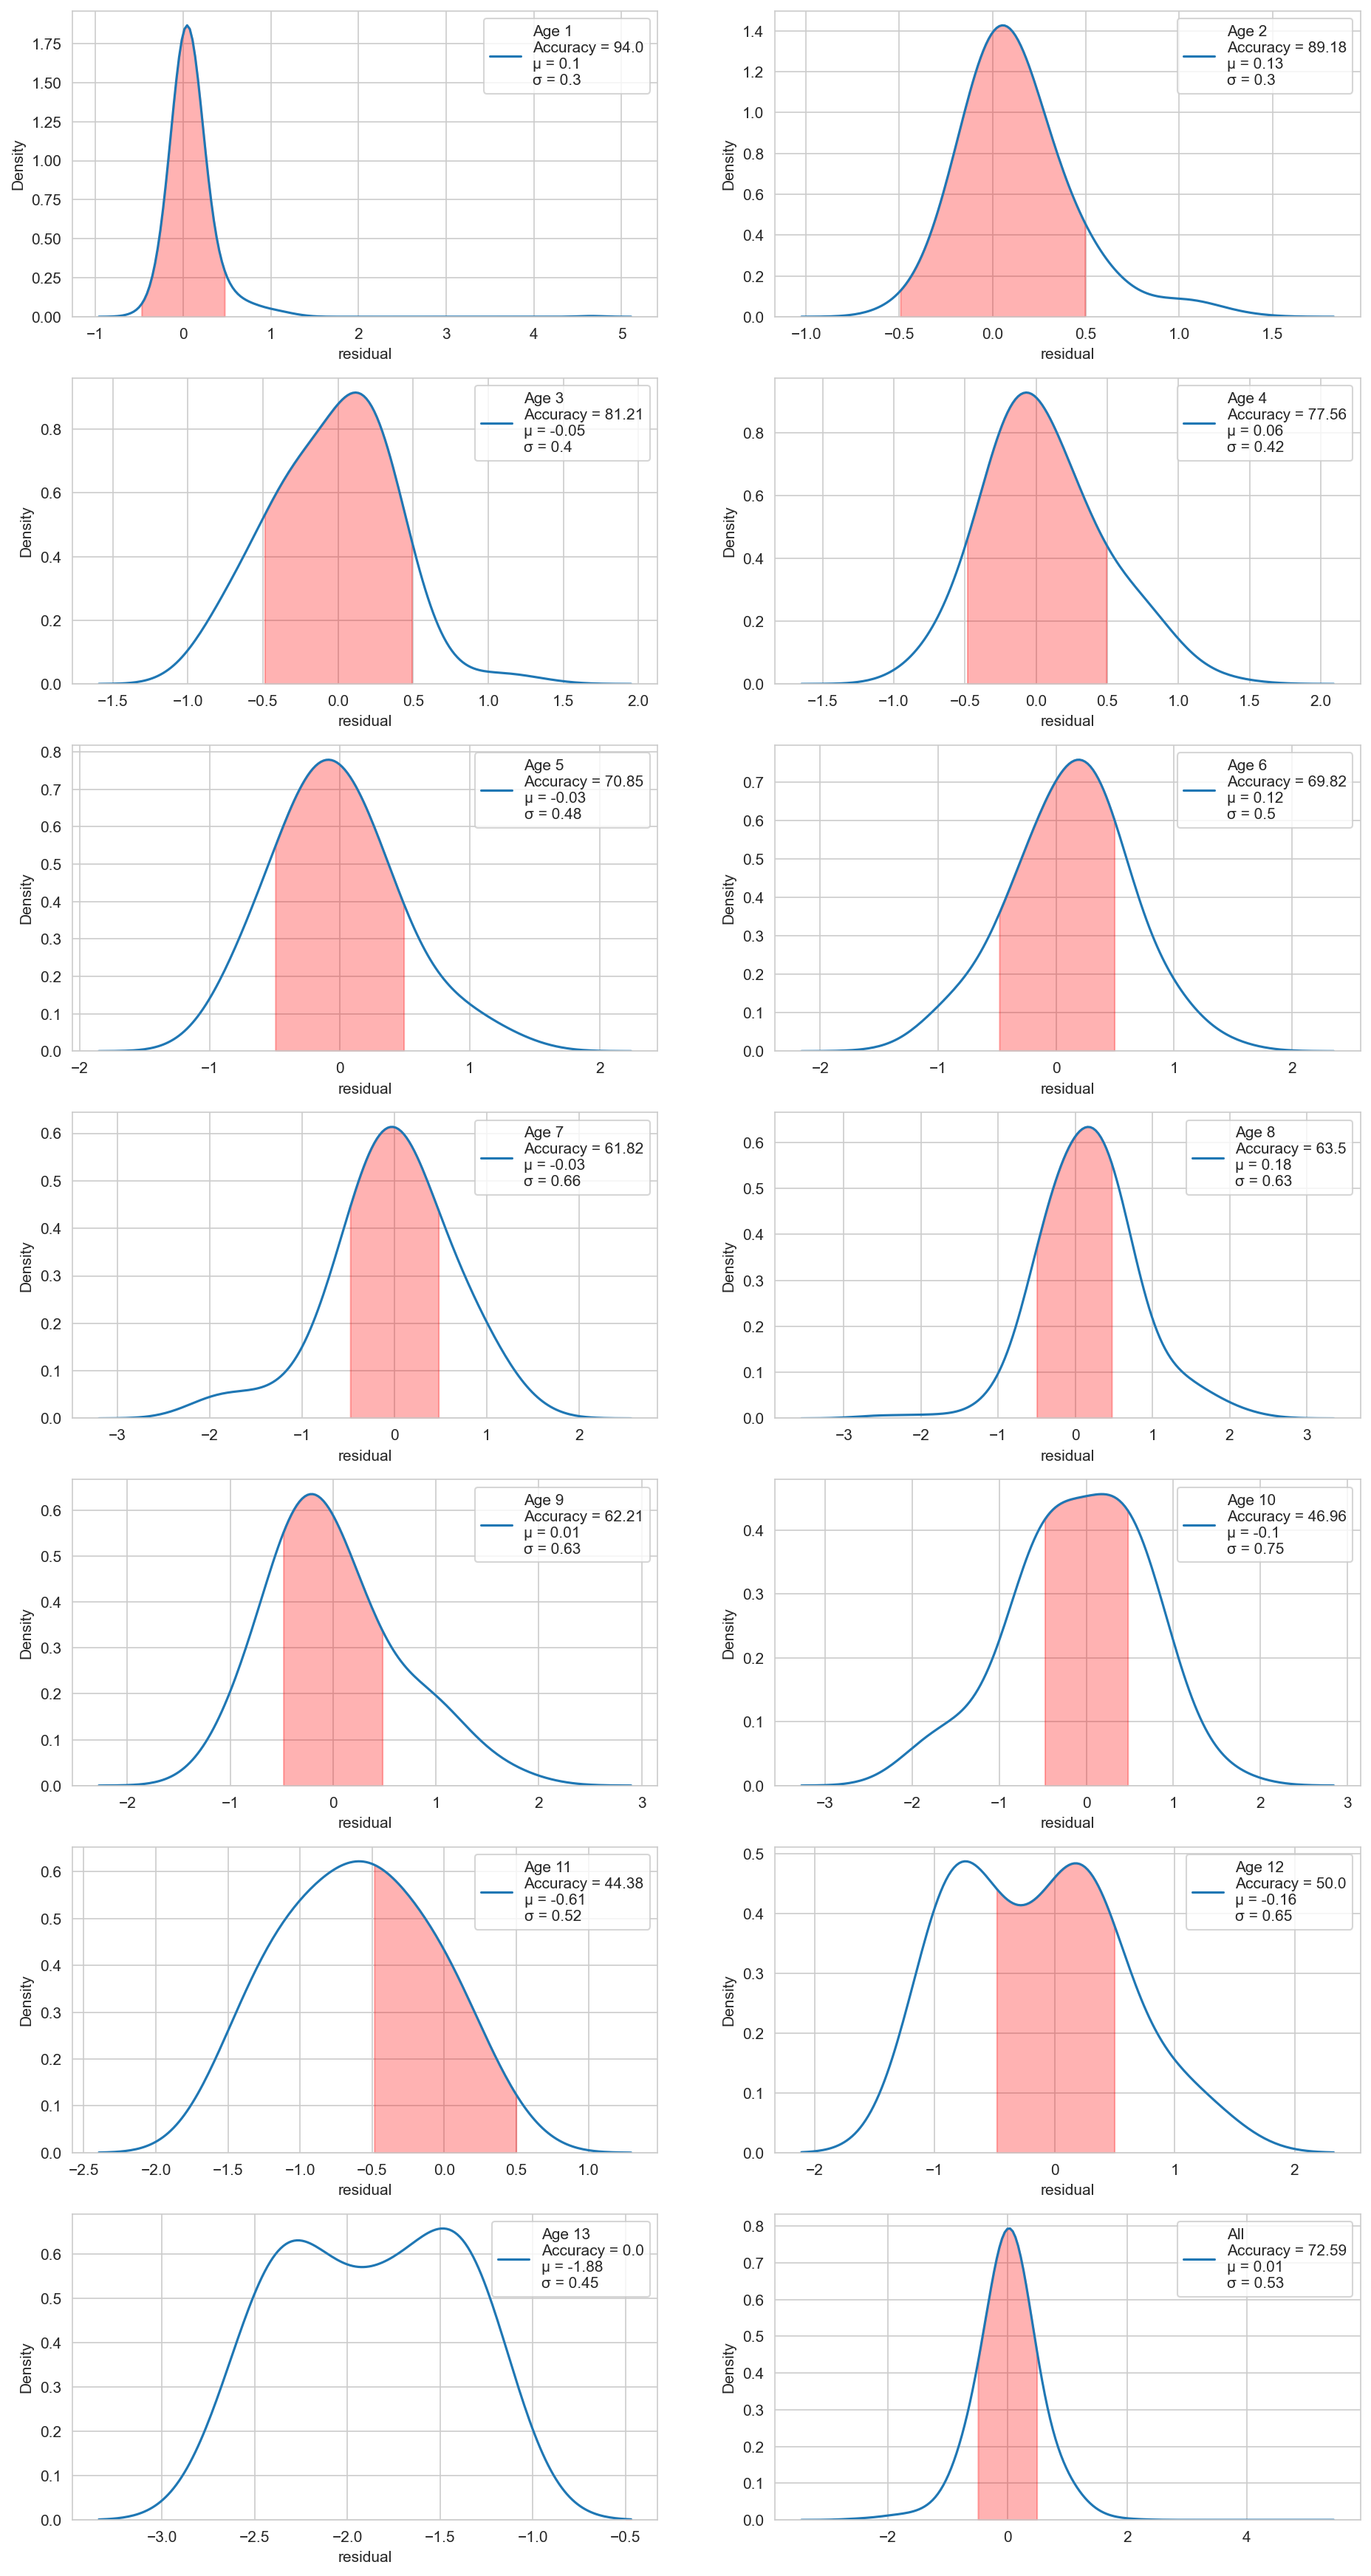
\includegraphics[scale=0.46]{results/eda/acc_by_age_dist.png}
  \label{age_acc}
\end{figure}

The figures below shows the predictions per age group on the test-set. We
can see that the prediction follows a linear trend $y=x$ except for the 2-3 last years,
when the mean drops below $y=x$. This is even more obvious in the residual plots
where the prediction drops below $y=0$ for the last 2-3 age groups.


\begin{figure}
  \centering
  \subfloat[B4 minimum exposure]{\label{ref_label1}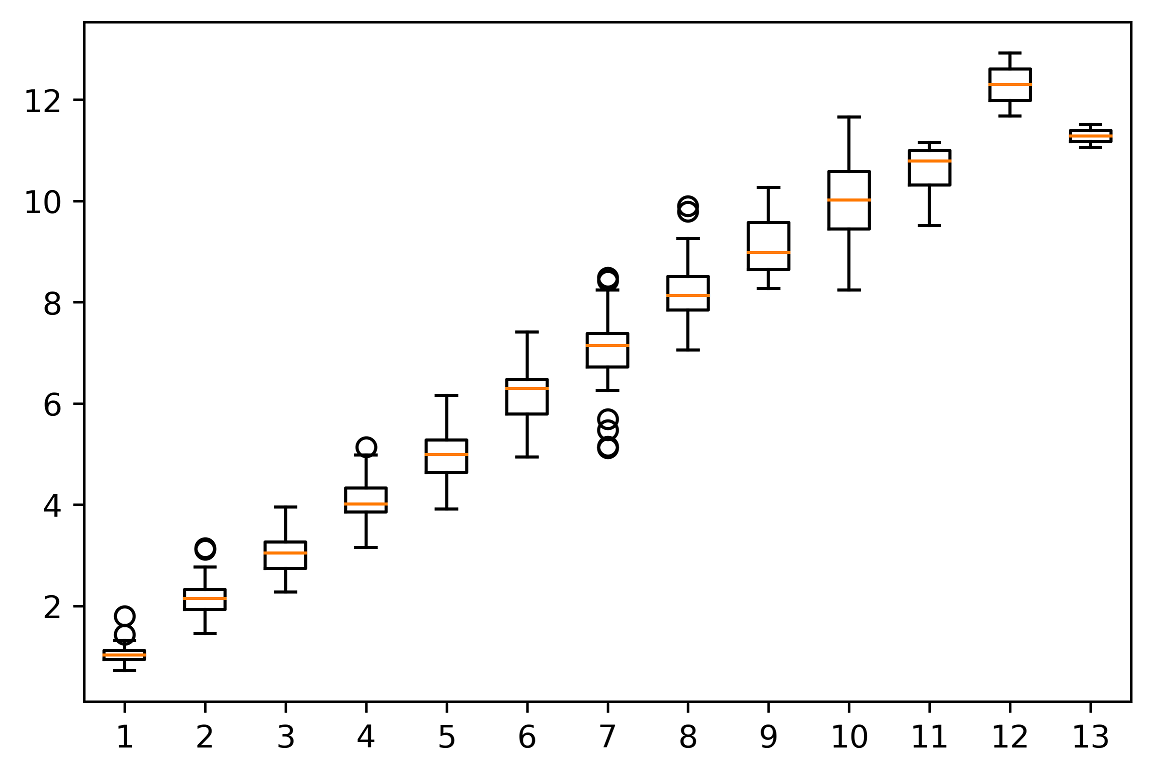
\includegraphics[width=0.5\textwidth]{result_pr_model/b4_min/boxplot_pr_age.png}}
  \subfloat[B4 minimum exposure residuals]{\label{ref_label2}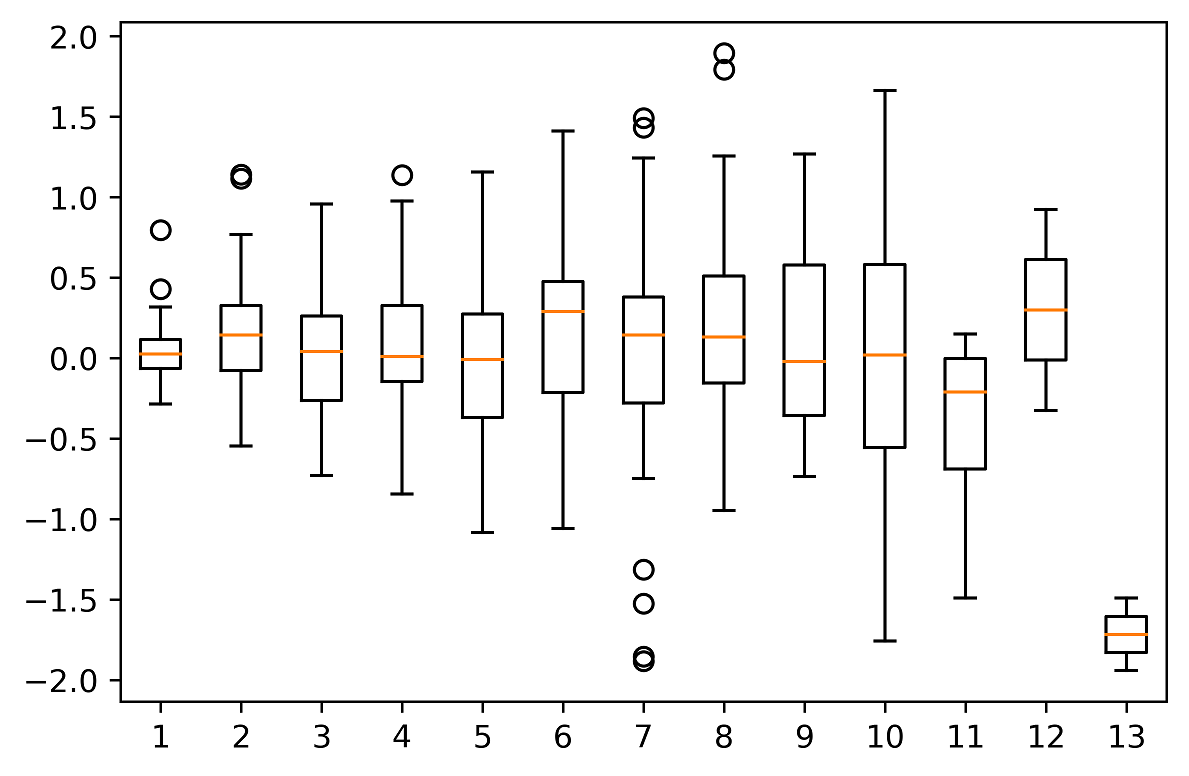
\includegraphics[width=0.5\textwidth]{result_pr_model/b4_min/boxplot_residual.png}}

  \subfloat[B5 minimum exposure]{\label{ref_label3}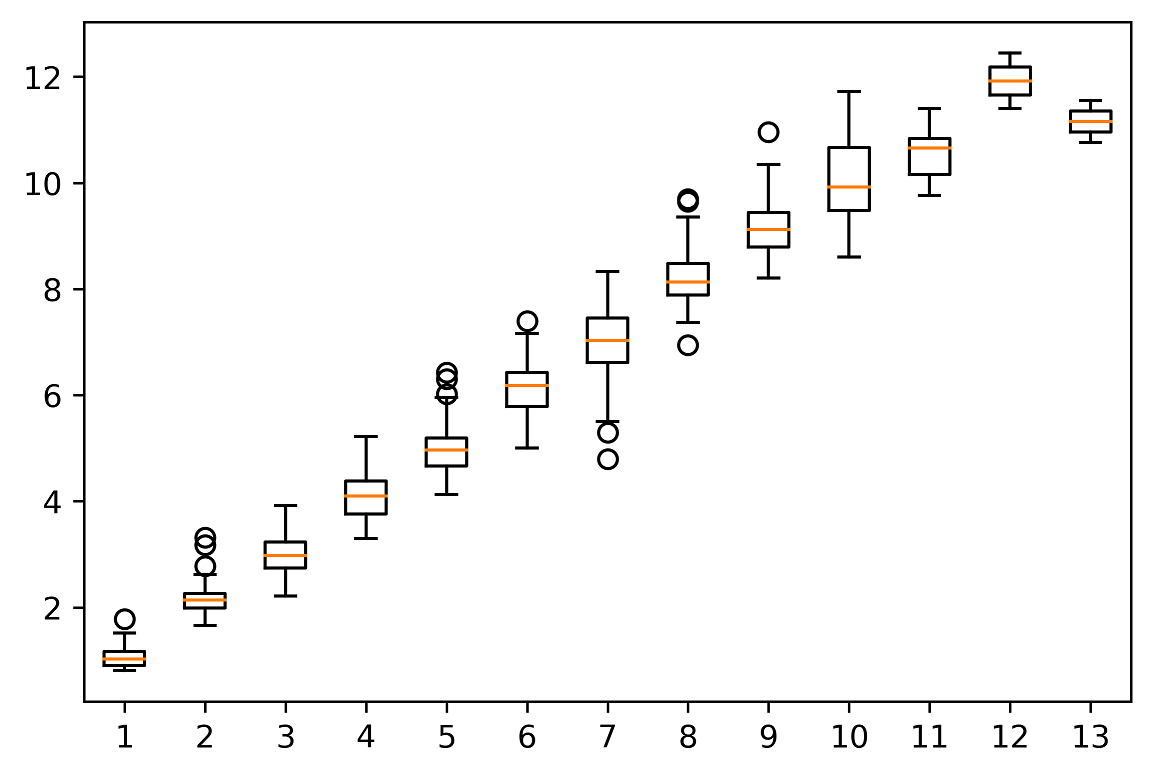
\includegraphics[width=0.5\textwidth]{result_pr_model/b5_min/boxplot_pr_age.png}}
  \subfloat[B5 minimum exposure, residuals]{\label{ref_label4}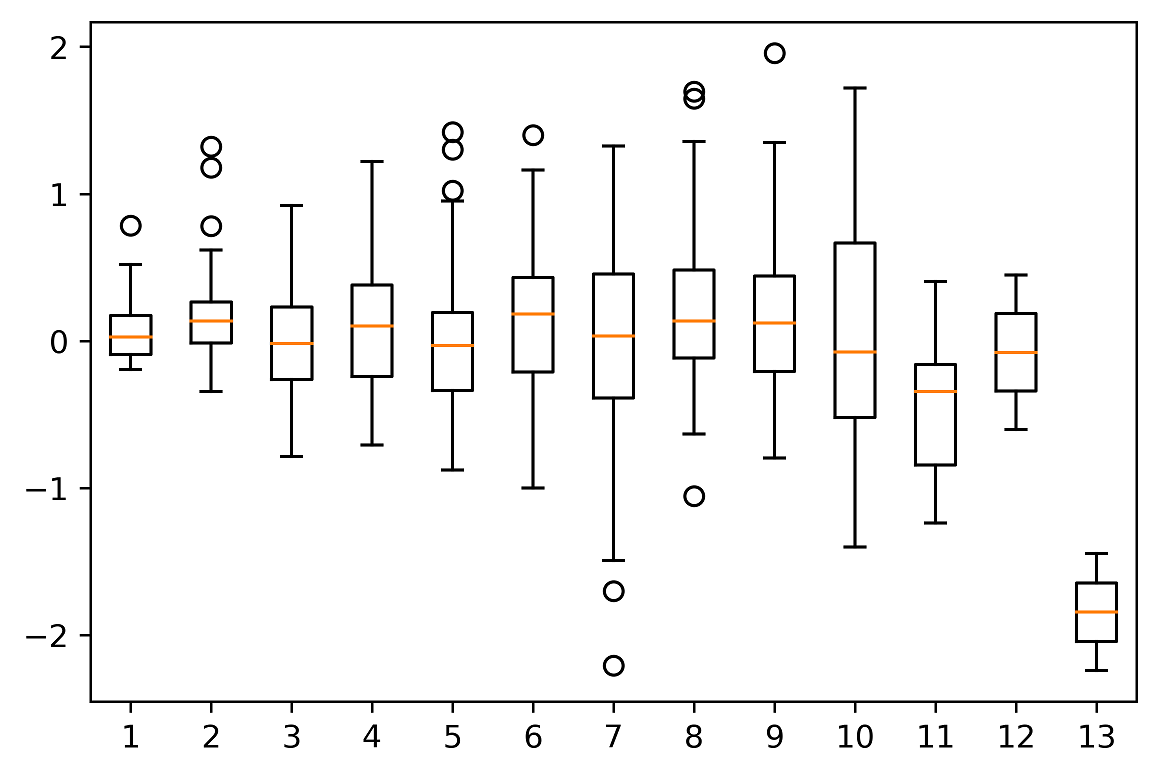
\includegraphics[width=0.5\textwidth]{result_pr_model/b5_min/boxplot_residual.png}}
  
  \subfloat[B6 minimum exposure]{\label{ref_label3}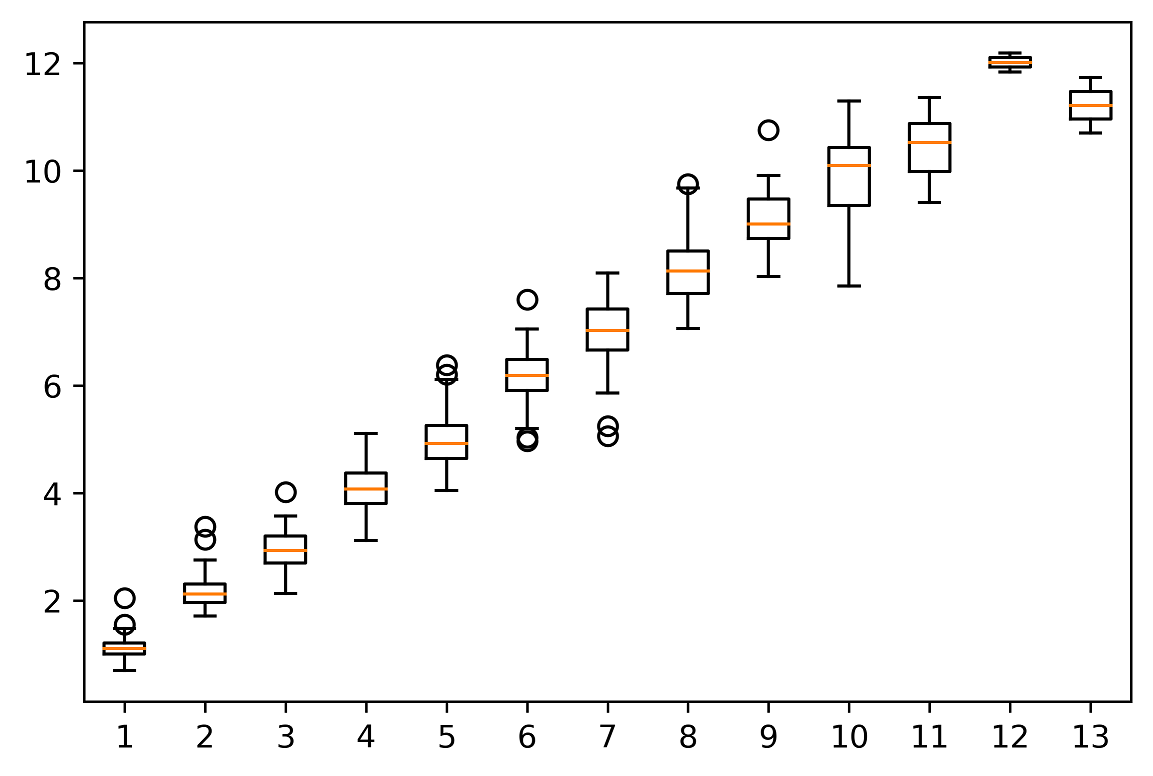
\includegraphics[width=0.5\textwidth]{result_pr_model/b6_min/boxplot_pr_age.png}}
  \subfloat[B6 minimum exposure, residuals]{\label{ref_label4}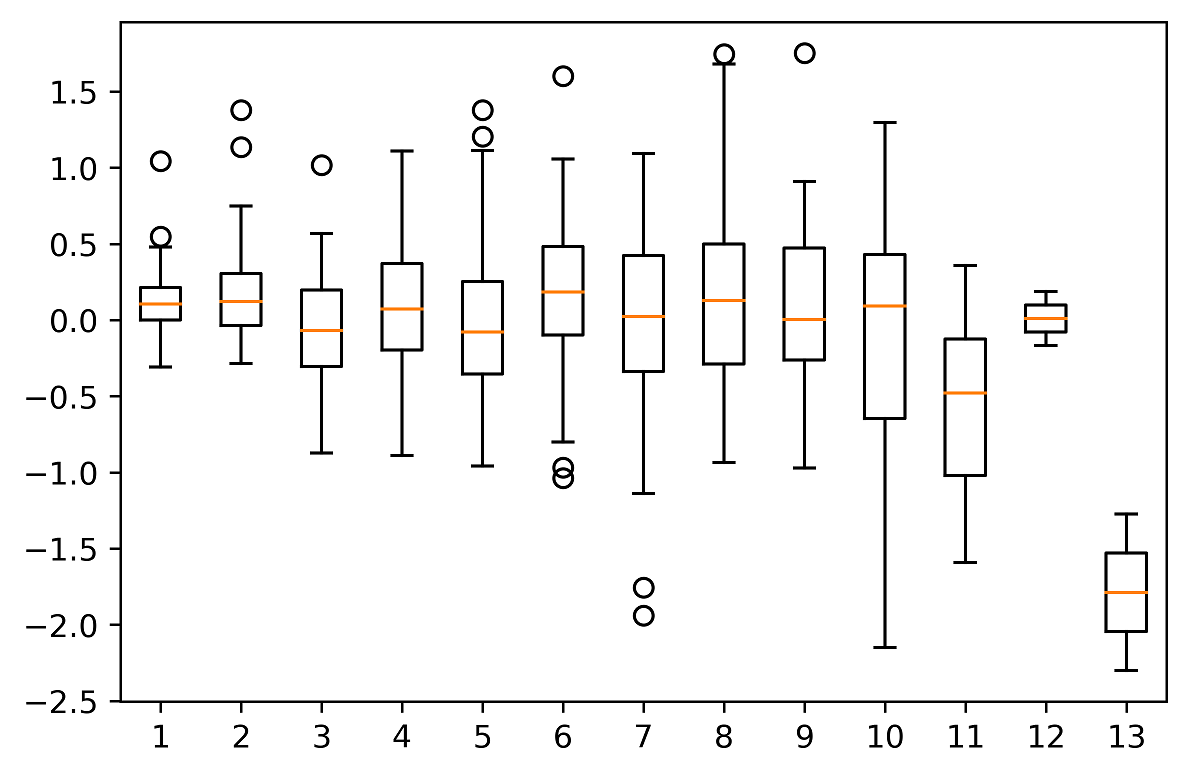
\includegraphics[width=0.5\textwidth]{result_pr_model/b6_min/boxplot_residual.png}}  
  \caption{\label{ref_label_overall}Comparing the models, looking at age per age class, and the residuals per prediction}
  \label{marker6}
\end{figure}

Figure \ref{marker7} shows scatter plots of all predictions that results in a miss-classification. That is predictions
that error greater than 0.5 in magnitude. Predictions that miss by more than 1.5 in magnitude are shown with red dots.

\begin{figure}
  \centering
  \subfloat[B4 minimum exposure]{\label{ref_label1}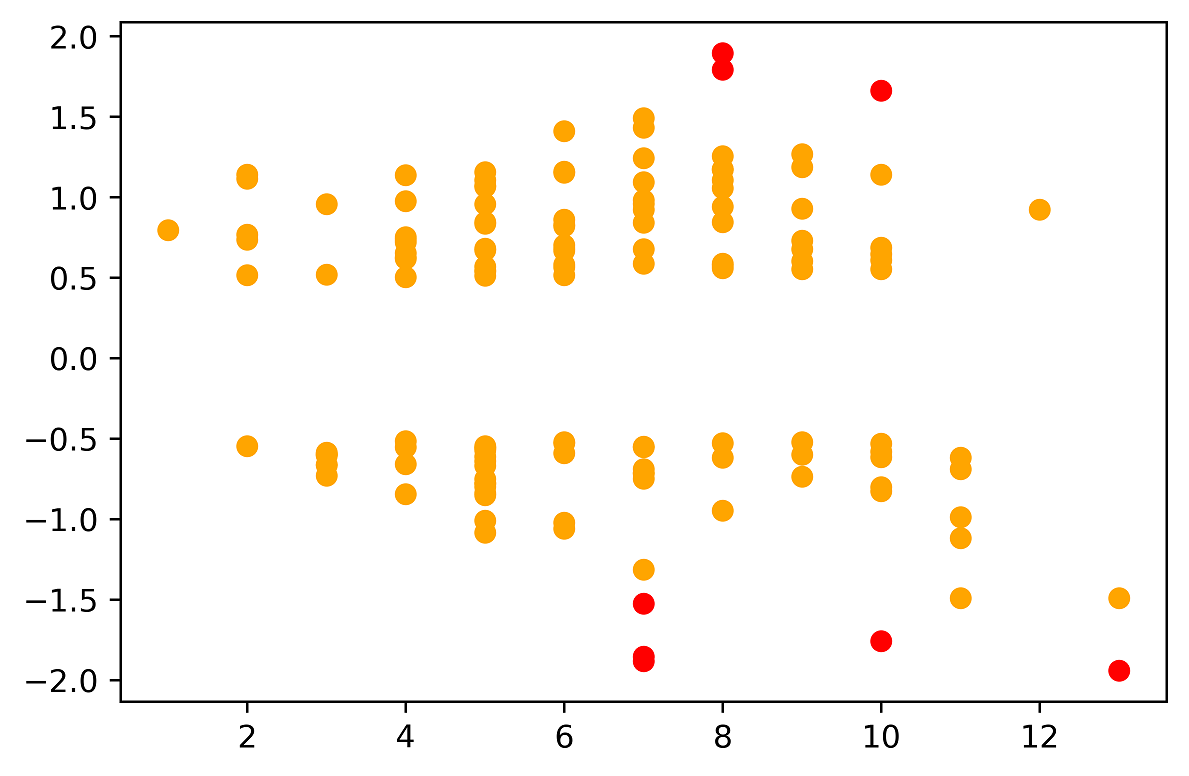
\includegraphics[width=0.5\textwidth]{result_pr_model/b4_min/misclassification.png}}

  \subfloat[B5 minimum exposure]{\label{ref_label3}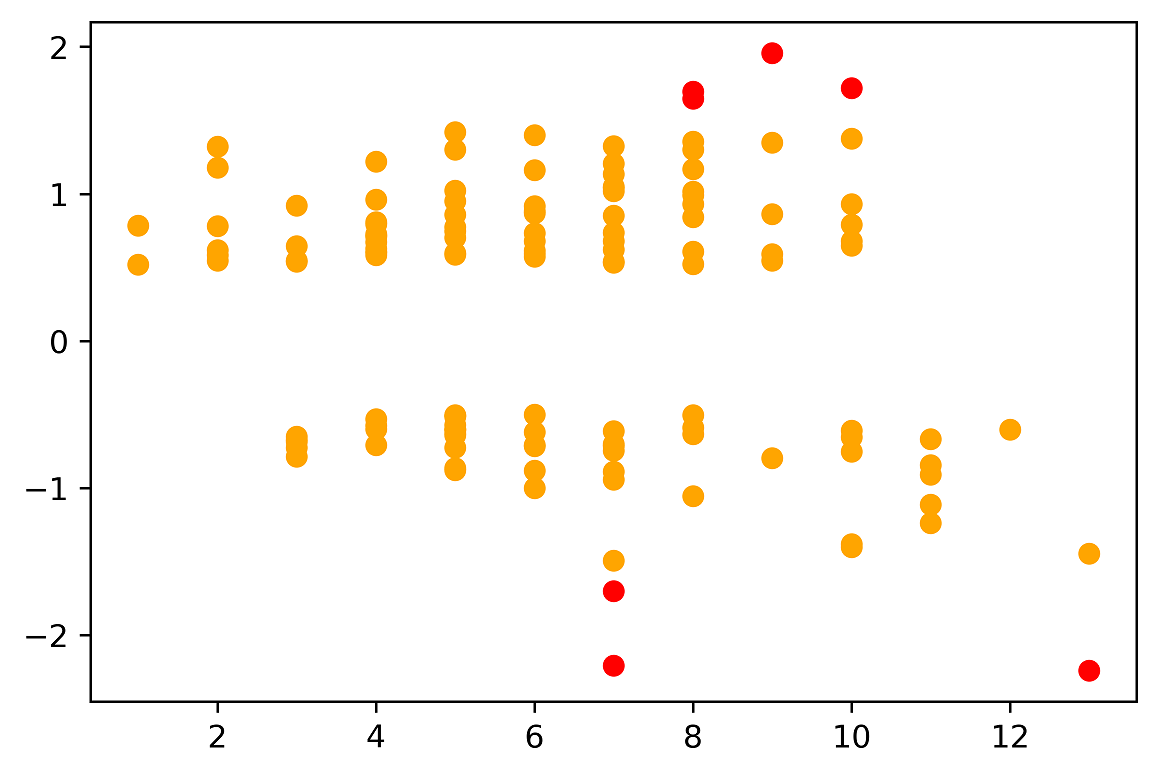
\includegraphics[width=0.5\textwidth]{result_pr_model/b5_min/misclassification.png}}
  
  \subfloat[B6 minimum exposure]{\label{ref_label3}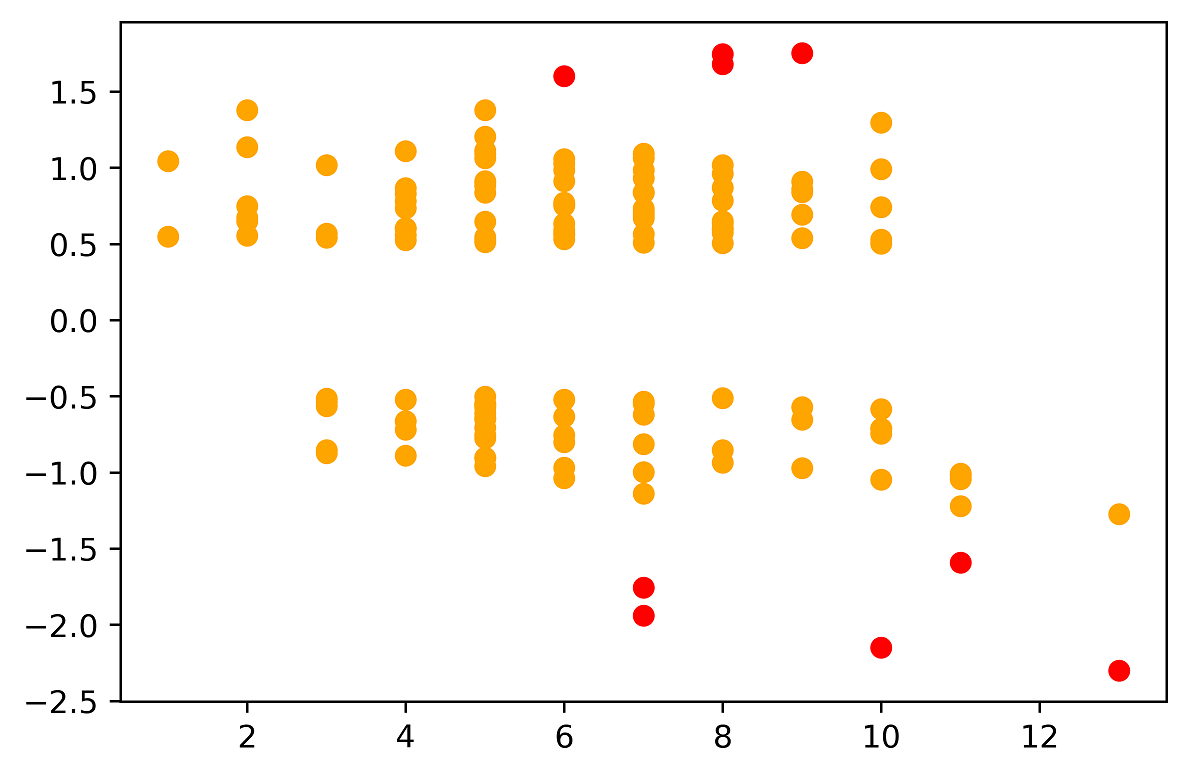
\includegraphics[width=0.5\textwidth]{result_pr_model/b6_min/misclassification.png}}
  \caption{\label{ref_label_overall}Comparing the models, looking at age per age class, and the reciduals per perdiction}
  \label{marker7}
\end{figure}


\subsection*{Ensemble of ensembles}

We search the space of ensemble of ensemble predictions
which are given by 
$\sum_{k=1}^{N}\binom{N}{k} $ where $N=22$ and $k \in 1..N$
and find three ensemble of ensembles which produce the best
results overall with accuracy of 75.9\%, 76.1\%, and 76.9\%
and MSE 0.247, 0.248, and 0.248 from ensemble of 
all networks, ensemble of B4, B5 and B6 with min exposure,
and ensemble of B4, B5, B6 and middle with min exposure.


\begin{figure}[h!]
  \begin{minipage}[b]{0.49\textwidth}
  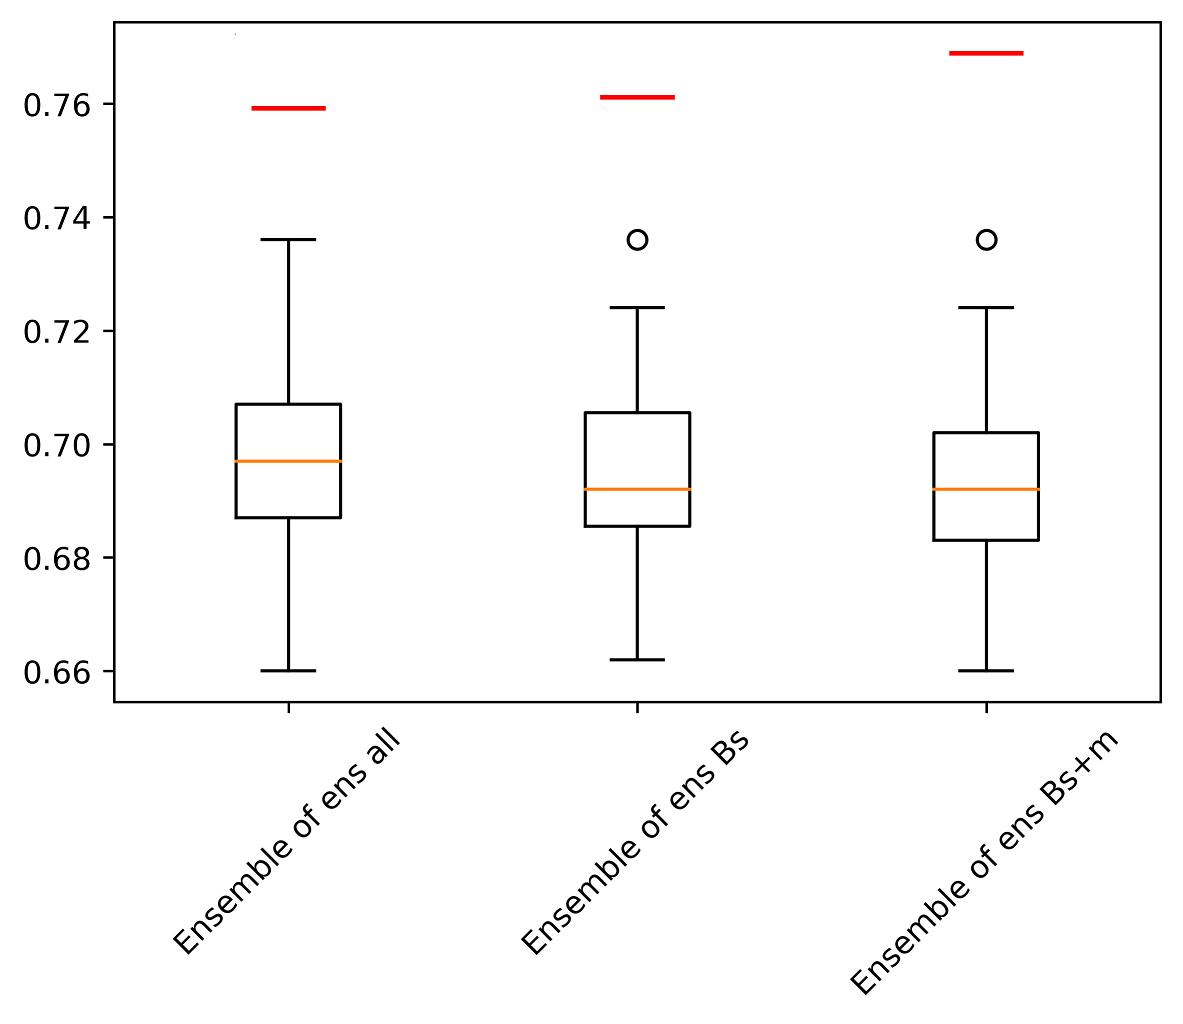
\includegraphics[scale=0.35]{results/eoe_acc.png}
    \caption{Ensemble of ensemble: accuracy of the 3 best models}
   \label{marker5}
  \end{minipage}
  \hfill
\end{figure}

\begin{figure}[h!]
  \begin{minipage}[b]{0.49\textwidth}
  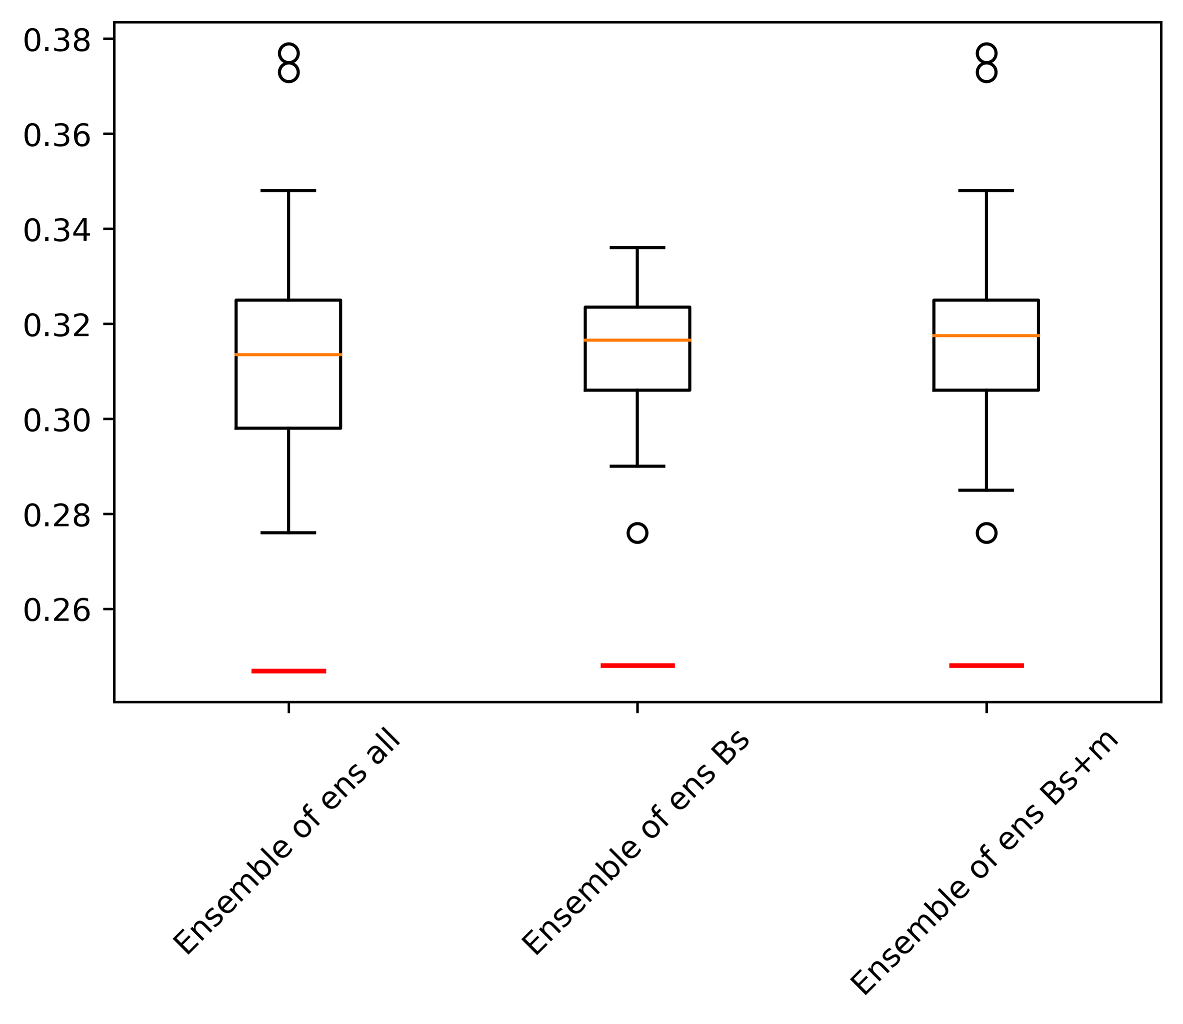
\includegraphics[scale=0.35]{results/eoe_mse.png}
    \caption{Ensemble of ensemble: mse of the 3 best models}
   \label{marker5}
  \end{minipage}
  \hfill
\end{figure}

\begin{center}
\begin{table}[hbt!]
\caption{Accuracy/MSE pr ensemble of ensemble.
Eoe1 is ensemble of ensemble of all models, Eoe2 is for B4, B5 and B6,
and Eoe3 is Eoe2 plus efficientNetV2 medium.}
\begin{tabular}{ |l|c|c|c| }
\hline
score/ensemble & eoe1 & eoe2 & eoe3  \\ \hline
Accuracy & 75.9 & 76.1 & 76.9 \\ 
MSE & .247 & .248 & .248  \\ 
\hline
\end{tabular}
\label{table10}
\end{table}
\end{center}

\subsection*{Outliers}

Looking at figure \ref{marker6} we can see that the model under-predicts the age of older otoliths. This pattern is especially observable for individuals read as 15 years and older. The oldest predication is 18 years while the test set contains individuals as old as 22 years. To better understand the bias, figure \ref{marker5} shows the 4 largest outliers from the test set which come from two pairs



\begin{figure}[h!]
  \caption{Some of the most common images with miss-predicted of more than 1.5 years}
  \centering
  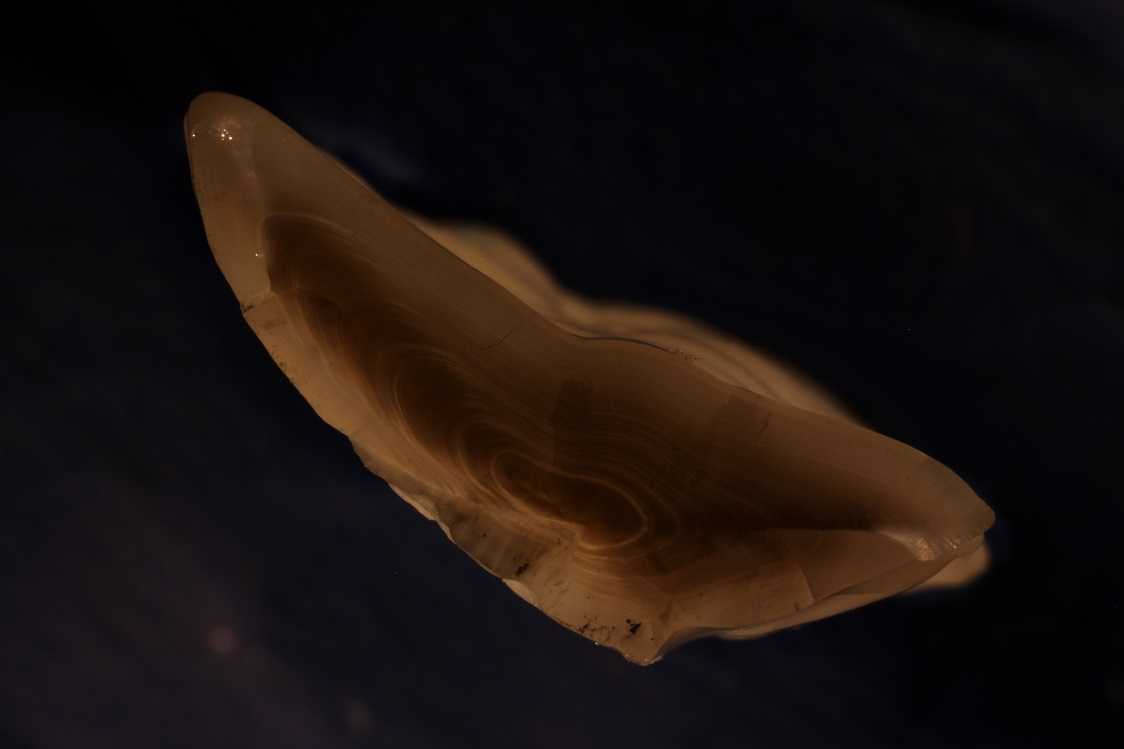
\includegraphics[scale=0.08]{outliers/IMG_0284_13.JPG}
  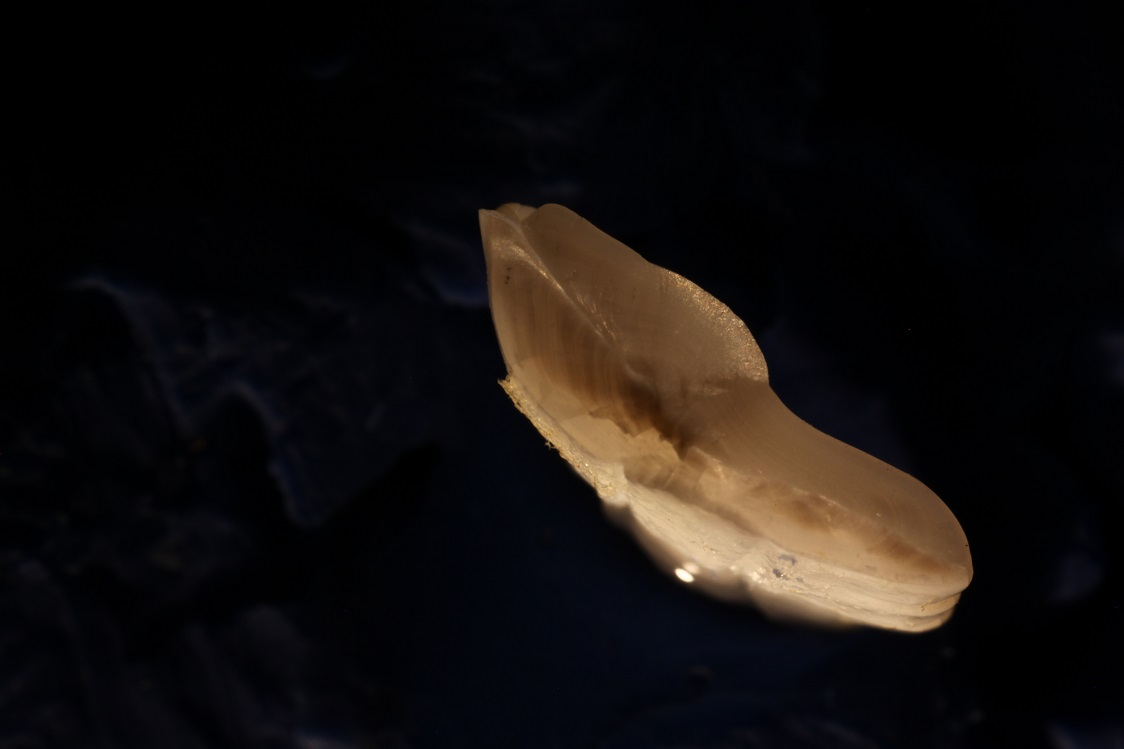
\includegraphics[scale=0.08]{outliers/IMG_0230_71.JPG}
  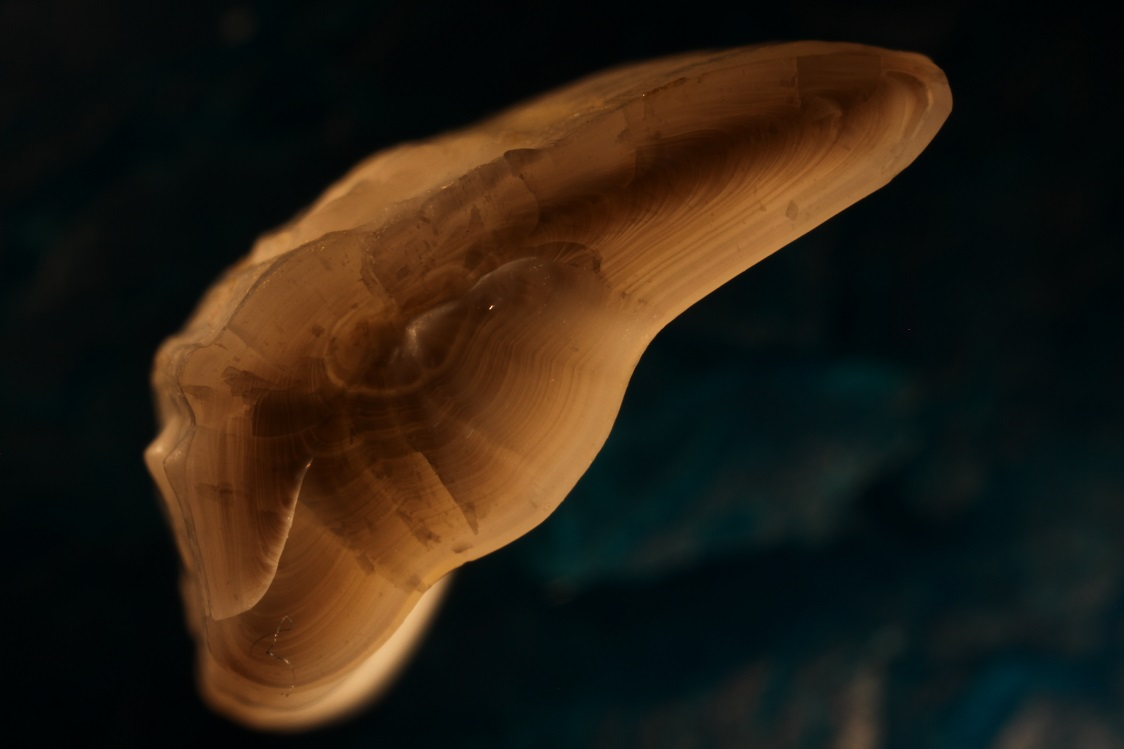
\includegraphics[scale=0.08]{outliers/IMG_0104_270.JPG} 

  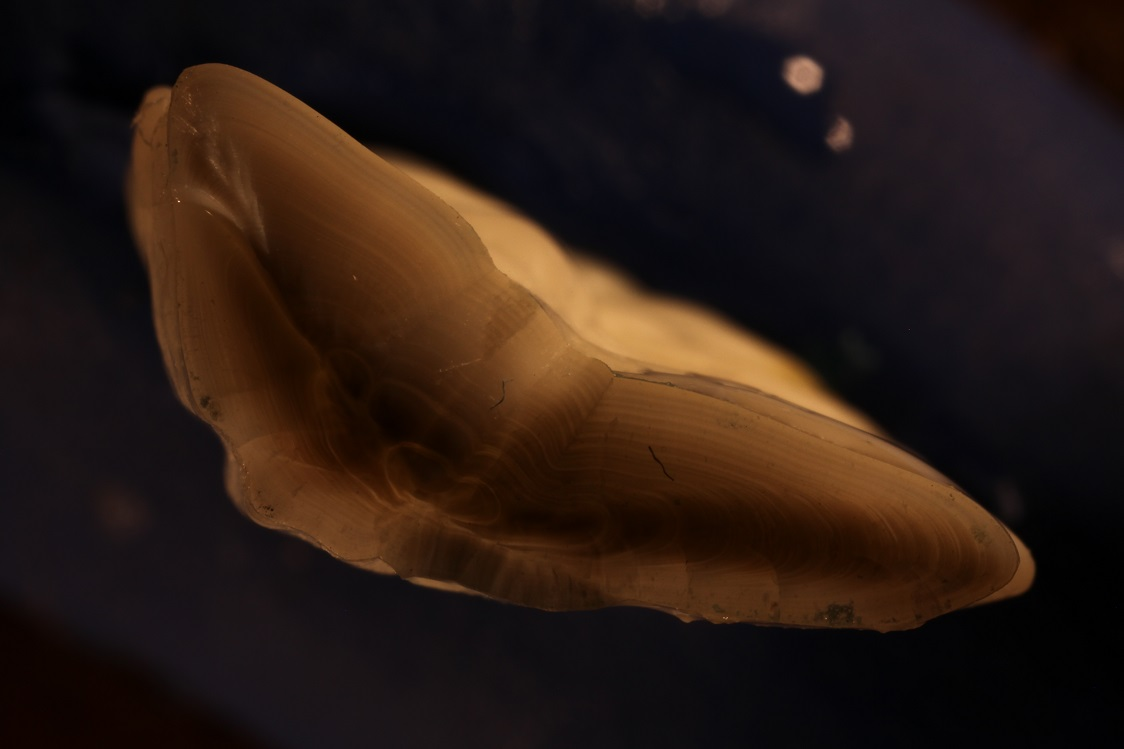
\includegraphics[scale=0.08]{outliers/IMG_0044_342.JPG}
  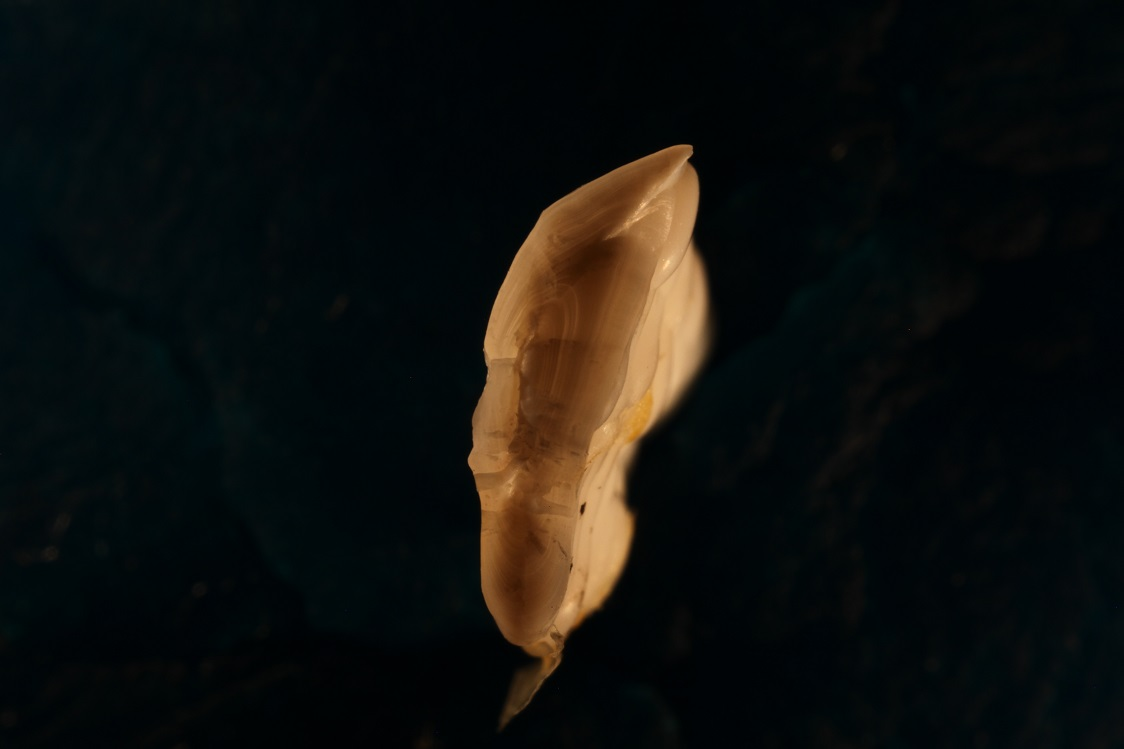
\includegraphics[scale=0.08]{outliers/IMG_0086_360.JPG}
  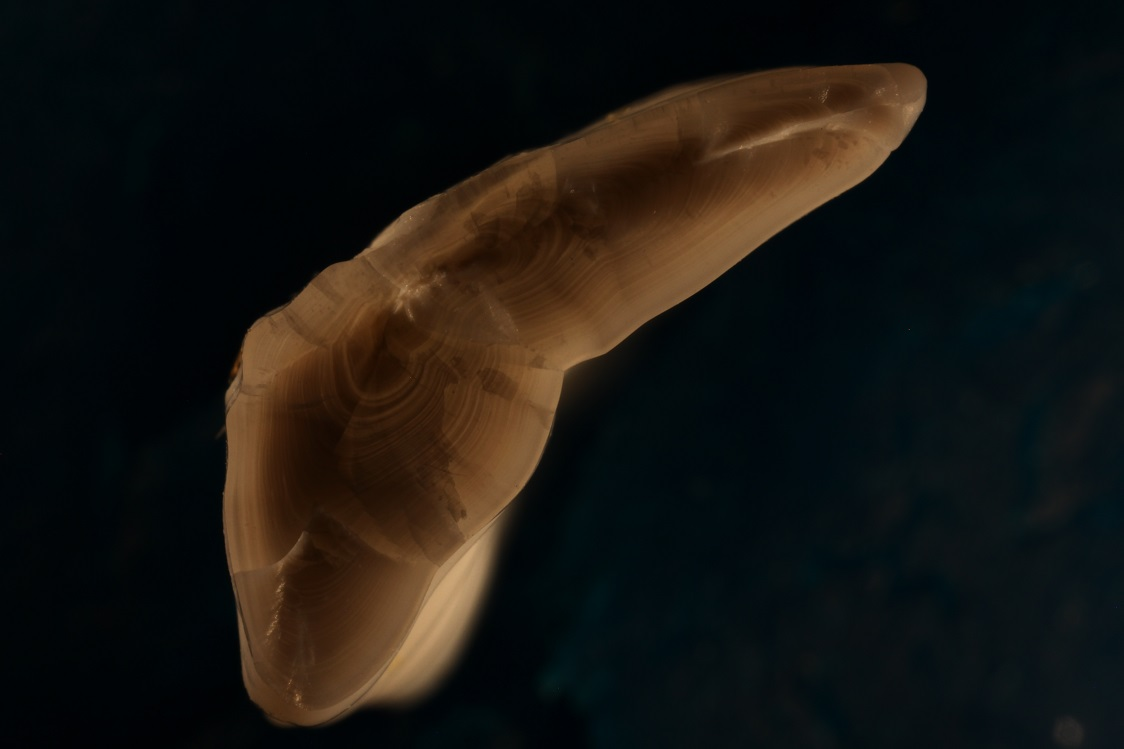
\includegraphics[scale=0.08]{outliers/IMG_0122_369.JPG}
  
  \label{marker10}
\end{figure}

Figure \ref{marker7} are the most commonly miss-classified images 
with greatest magnitude of error.

\subsection*{Correlation of predictions across models}

From the outliers we can see there is a correlation of predicting outliers across models. 
Lets look at the correlation of models on the test-set predictions.

\begin{figure}[h!]
  \caption{Pearson correlation of each model prediction on the test-set}
  \centering
  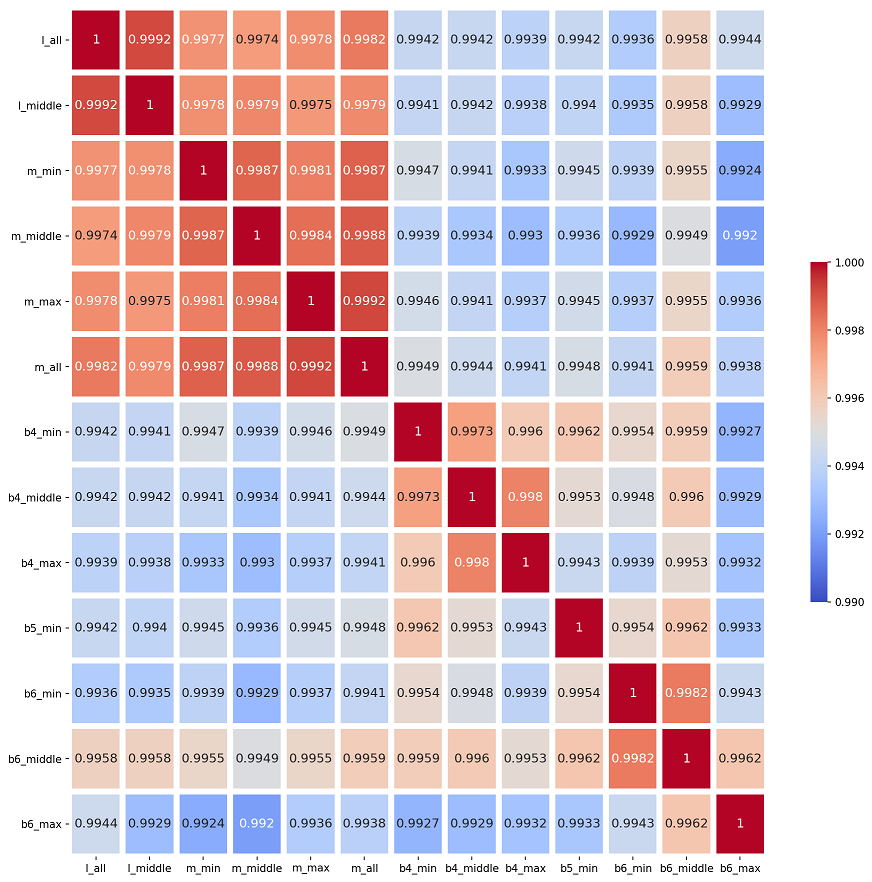
\includegraphics[scale=0.5]{results/eda/pearson_corr_models.png}
  \label{marker11}
\end{figure}

We can see that EfficientNetV2 models are most correlated to each other, and that B4 models are correlated.
Also B6 on middle exposure is correlated to all models. All the results are highly correlations. 

We can also look at the correlation between models pr age-class.
\begin{figure}[h!]
  \caption{Scatter plot of each age-class by Large-all $\times$ Large-medium}
  \centering
  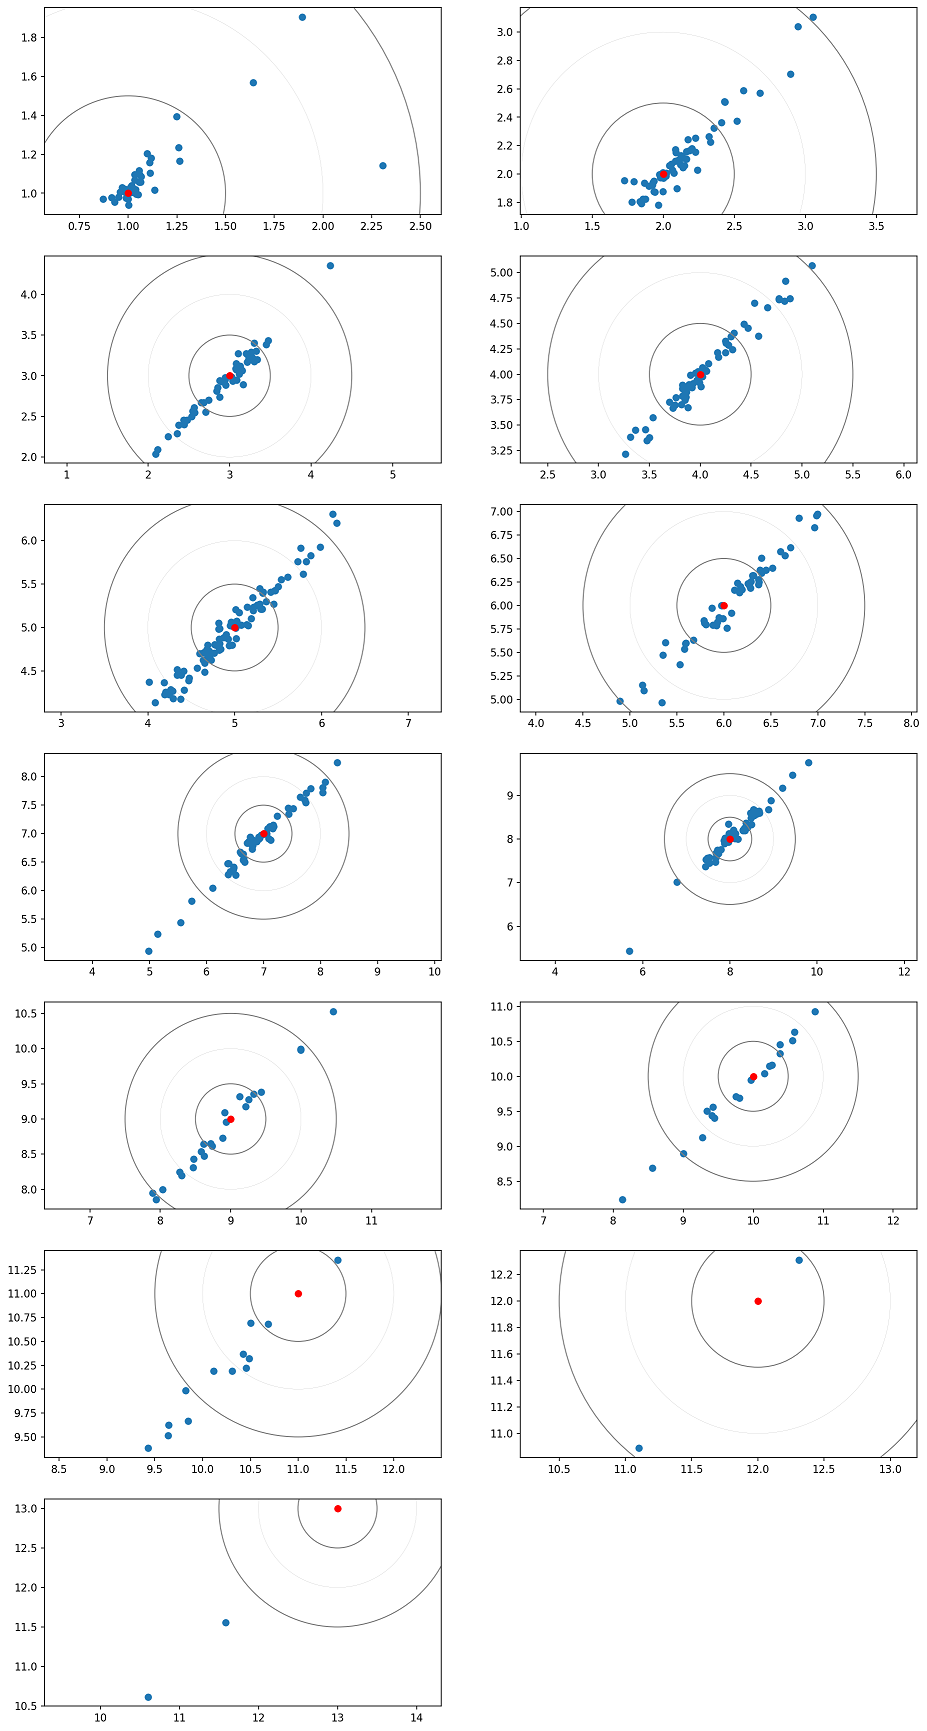
\includegraphics[scale=0.45]{results/eda/l_all_x_l_middle.png}
  \label{marker11}
\end{figure}



\section*{Discussion}

During initial training we trained a B4 network on ca 2000 images and obtained
an accuracy of ca 60\%, later another 3000 images was added and the same
network was trained on ca 5000 images which resulted in accuracy of ca 70\%.
It could be interesting to investigating if adding another 3-5000 images
would increase the accuracy to 80\%.


\section*{References}

\bibliographystyle{apalike}
\bibliography{references}

\appendix
\section{\\Common outliers of more than 1.5 years}
% the \\ insures the section title is centered below the phrase: AppendixA

\begin{table}[!ht]
    \centering
    \caption{Outliers with more than 1.5 year error. Index of image in test-set per model}
    \begin{tabular}{|l|l|l|l|l|l|l|l|}
    \hline
        V2-m,mid. & V2-m,mid. & V2-l,all & V2-l,mid. & B4,min & B5,min &  B6,min & B6,mid.  \\ \hline
        ~ & ~ & ~ & ~ & 13 & 13 & 13 & 13  \\ \hline
        ~ & ~ & ~ & ~ & ~ & ~ & 48 &   \\ \hline
        71 & 71 & 71 & 71 & 71 & 71 & 71 & 71  \\ \hline
        92 & 92 & ~ & ~ & ~ & ~ & ~ &   \\ \hline
        ~ & ~ & ~ & ~ & 270 & 270 & ~ & 270  \\ \hline
        279 & 279 & 279 & 279 & 279 & 279 & 279 & 279  \\ \hline
        ~ & ~ & 312 & 312 & ~ & ~ & ~ &   \\ \hline
        ~ & ~ & ~ & 320 & 320 & ~ & ~ &   \\ \hline
        362 & 362 & 362 & 362 & 362 & 362 & 362 & 362  \\ \hline
        342 & 342 & 342 & 342 & 342 & 342 & 342 & 342  \\ \hline
        369 & 369 & 369 & 369 & 369 & ~ & 369 & 369  \\ \hline
        ~ & ~ & ~ & 393 & ~ & ~ & 393 & 393  \\ \hline
        423 & 423 & 423 & 423 & ~ & ~ & ~ &   \\ \hline
        ~ & ~ & ~ & ~ & ~ & 444 & ~ &   \\ \hline
        ~ & ~ & ~ & ~ & ~ & ~ & 502 & 502  \\ \hline
        ~ & ~ & ~ & ~ & ~ & ~ & ~ &   \\ \hline
        7 & 7 & 7 & 9 & 8 & 7 & 9 & 9  \\ \hline
    \end{tabular}
\end{table}

\begin{table}[!ht]
    \centering
    \caption{Outliers with more than 1.5 year error. Prediction and true age, per model}
    \begin{tabular}{|l|l|l|l|l|l|l|l|l|}
    \hline
        Idx & V2-m,mid. & V2-l,all & V2-l,mid. & B4,min & B5,min &  B6,min & B6,mid. & Age  \\ \hline
        13 & ~ & ~ & ~ & 9.79 & 9.64 & 9.74 & 9.58 & 8  \\ \hline
        48 & ~ & ~ & ~ & ~ & ~ & 7.6 & ~ & 6  \\ \hline
        71 & 4.96 & 4.98 & 4.94 & 5.14 & 4.79 & 5.06 & 5.12 & 7  \\ \hline
        92 & 10.95 & ~ & ~ & ~ & ~ & ~ & ~ & 13  \\ \hline
        270 & ~ & ~ & ~ & 11.66 & 11.71 & ~ & 11.53 & 10  \\ \hline
        279 & 9.93 & 9.79 & 9.75 & 9.89 & 9.69 & 9.67 & 9.7 & 8  \\ \hline
        312 & ~ & 9.42 & 9.38 & ~ & ~ & ~ & ~ & 11  \\ \hline
        320 & ~ & ~ & 5.44 & 5.47 & ~ & ~ & ~ & 7  \\ \hline
        362 & 5.11 & 5.14 & 5.23 & 5.11 & 5.29 & 5.24 & 5.15 & 7  \\ \hline
        342 & 10.35 & 10.6 & 10.61 & 11.05 & 10.75 & 10.69 & 10.84 & 13  \\ \hline
        369 & 8.17 & 8.13 & 8.23 & 8.24 & ~ & 7.85 & 8.29 & 10  \\ \hline
        393 & ~ & ~ & 10.53 & ~ & ~ & 10.75 & 10.83 & 9  \\ \hline
        423 & 5.39 & 5.69 & 5.43 & ~ & ~ & ~ & ~ & 8  \\ \hline
        444 & ~ & ~ & ~ & ~ & 10.95 & ~ & ~ & 9  \\ \hline
        502 & ~ & ~ & ~ & ~ & ~ & 9.4 & 9.43 & 11  \\ \hline
    \end{tabular}
\end{table}

\section{\\Mean and standard deviation per model x per Age group}
% the \\ insures the section title is centered below the phrase: Appendix B

\begin{figure}[h!]
  \caption{Mean of residuals per age-group}
  \centering
  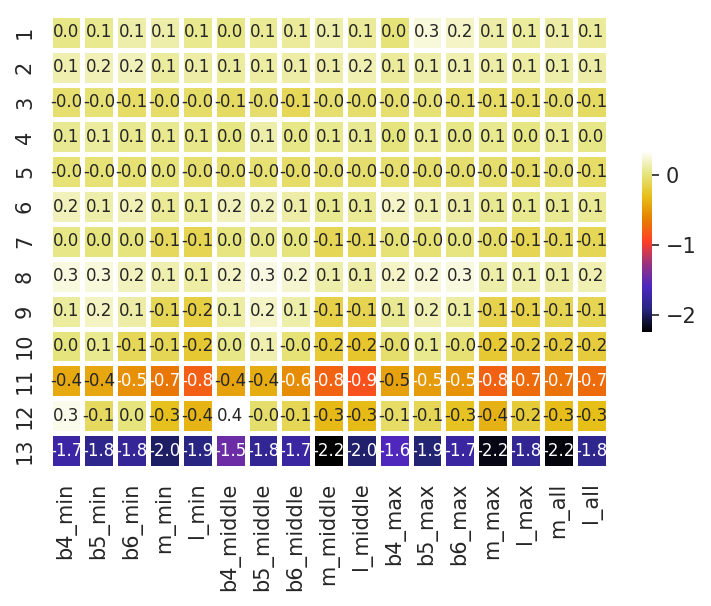
\includegraphics[scale=0.5]{results/eda/age_mean.png}
  \label{age_acc}
\end{figure}

\begin{figure}[h!]
  \caption{Standard deviation of residuals per age-group}
  \centering
  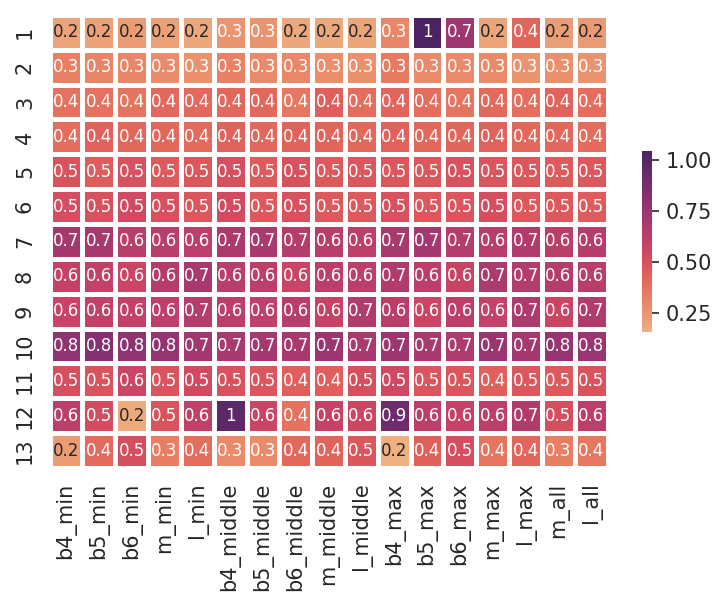
\includegraphics[scale=0.5]{results/eda/age_std.png}
  \label{age_acc}
\end{figure}

\section{\\Accuracy and MSE per model and per fold}

\begin{table}[!ht]
    \caption{MSE per CNN and per fold}
    \centering
    \begin{tabular}{|l|l|l|l|l|l|l|l|l|l|l|l|l|}
    \hline
        CNN/fold & 1 & 2 & 3 & 4 & 5 & 6 & 7 & 8 & 9 & 10 & ens. \\ \hline
        B4, min & .320 & .318 & .306 & .313 & .322 & .314 & .315 & .316 & .306 & .302 & .277 \\ \hline
        B4, middle & .344 & .328 & .316 & .334 & .326 & .320 & .355 & .326 & .313 & .325 & .285 \\ \hline
        B4, max & .340 & .317 & .318 & .347 & .336 & .336 & .336 & .320 & .354 & .336 & .291 \\ \hline
        B5, min & .324 & .322 & .325 & .336 & .291 & .314 & .320 & .331 & .33 & .317 & .277 \\ \hline
        B5, middle & ~ & ~ & ~ & ~ & ~ & ~ & ~ & ~ & ~ & ~ & ~ \\ \hline
        B5, max & ~ & ~ & ~ & ~ & ~ & ~ & ~ & ~ & ~ & ~ & ~ \\ \hline
        B6, min & .325 & .329 & .334 & .293 & .312 & .290 & .320 & .300 & .276 & .306 & .272 \\ \hline
        B6, middle & .323 & .301 & .312 & .268 & .294 & .266 & .309 & .311 & .278 & .289 & .262 \\ \hline
        B6, max & .435 & .306 & .306 & .270 & .390 & .321 & .411 & .321 & .294 & .448 & .305 \\ \hline
        medium, min & .292 & .292 & .294 & .275 & .298 & .304 & .304 & .331 & .307 & .295 & .273 \\ \hline
        med., mid. & .321 & .377 & .332 & .285 & .285 & .325 & .311 & .348 & .295 & .373 & .292 \\ \hline
        medium, max & .305 & .413 & .319 & .327 & .310 & .284 & .309 & .315 & .302 & .287 & .290 \\ \hline
        medium, all & .292 & .289 & .289 & .326 & .307 & .327 & .283 & .300 & .335 & .295 & .281 \\ \hline
        large, min & ~ & ~ & ~ & ~ & ~ & ~ & ~ & ~ & ~ & ~ & ~ \\ \hline
        large, middle & .301 & .281 & .299 & .318 & .282 & .305 & .280 & .334 & .3 & .310 & .280 \\ \hline
        large, max & ~ & ~ & ~ & ~ & ~ & ~ & ~ & ~ & ~ & ~ & ~ \\ \hline
        large, all & .292 & .289 & .289 & .326 & .307 & .327 & .283 & .30 & .335 & .295 & .281 \\ \hline
    \end{tabular}
\label{table8}    
\end{table}

\begin{table}[!ht]
    \centering
    \caption{Accuracy per CNN and per fold}
    \begin{tabular}{|l|l|l|l|l|l|l|l|l|l|l|l|}
    \hline
        CNN/fold & 1 & 2 & 3 & 4 & 5 & 6 & 7 & 8 & 9 & 10 & ens. \\ \hline
        B4, min & 69.9 & 68.9 & 68.7 & 68.3 & 68.9 & 70.1 & 69.7 & 66.8 & 68.9 & 72.4 & 72.8 \\ \hline
        B4, middle & 68.5 & 69.3 & 73.0 & 68.5 & 67.8 & 68.2 & 67.2 & 67.2 & 68.3 & 69.5 & 71.5 \\ \hline
        B4, max & 64.1 & 68.2 & 67.2 & 66.2 & 67.8 & 69.5 & 67.2 & 69.3 & 66.2 & 65.2 & 70.9 \\ \hline
        B5, min & 71.8 & 69.1 & 69.3 & 66.8 & 73.6 & 70.7 & 66.2 & 68.3 & 69.5 & 68.7 & 74.4 \\ \hline
        B5, middle & ~ & ~ & ~ & ~ & ~ & ~ & ~ & ~ & ~ & ~ & ~ \\ \hline
        B5, max & ~ & ~ & ~ & ~ & ~ & ~ & ~ & ~ & ~ & ~ & ~ \\ \hline
        B6, min & 68.3 & 68.5 & 66.4 & 72.4 & 70.7 & 70.9 & 69.3 & 69.3 & 72.0 & 68.9 & 73.4 \\ \hline
        B6, middle & 68.5 & 69.9 & 67.6 & 73.6 & 72.8 & 72 & 68 & 69.3 & 72 & 71.1 & 74.4 \\ \hline
        B6, max & 70.5 & 68.2 & 65.2 & 73.2 & 69.1 & 67.8 & 68.0 & 68.0 & 72.8 & 68.5 & 71.5 \\ \hline
        medium, min & 71.1 & 71.1 & 69.5 & 73.4 & 71.8 & 70.9 & 70.9 & 69.7 & 70.1 & 71.5 & 74.0 \\ \hline
        med., mid. & 68.7 & 67.6 & 68.3 & 71.1 & 70.1 & 70.5 & 69.9 & 68.3 & 69.9 & 66 & 72.4 \\ \hline
        medium, max & 68.9 & 62.5 & 66.8 & 70.5 & 68.9 & 70.9 & 69.3 & 70.7 & 69.7 & 72.6 & 71.1 \\ \hline
        medium, all & 71.7 & 70.7 & 69.3 & 71.3 & 71.8 & 71.8 & 71.3 & 71.7 & 71.1 & 70.7 & 74.0 \\ \hline
        large, min & ~ & ~ & ~ & ~ & ~ & ~ & ~ & ~ & ~ & ~ & ~ \\ \hline
        large, middle & 69.7 & 73.4 & 69.1 & 67 & 71.8 & 69.9 & 72.6 & 68.2 & 70.5 & 70.3 & 71.8 \\ \hline
        large, max & ~ & ~ & ~ & ~ & ~ & ~ & ~ & ~ & ~ & ~ & ~ \\ \hline
        large, all & 70.9 & 70.7 & 70.5 & 70.7 & 71.5 & 69.3 & 70.7 & 71.8 & 69.7 & 70.9 & 71.7 \\ \hline
    \end{tabular}
\label{table9}    
\end{table}

\end{document}
